\documentclass[]{report}

\usepackage[a4paper, total={6in, 8in}]{geometry}
\usepackage{amsfonts}
\usepackage{amsmath}
\usepackage{amsthm}
\usepackage{hyperref}
\usepackage{tikz}
\usepackage{graphicx}
\usepackage{float}
\usepackage[boxruled,linesnumbered]{algorithm2e}
\usepackage{multirow}
\usepackage{cleveref}
\usepackage{wrapfig}
\usepackage{caption}
\usepackage{subcaption}
\usepackage{enumitem}
\usepackage{adjustbox}
\usepackage{pifont}

\theoremstyle{plain}
\newtheorem{theorem}{Theorem}[section]
\newtheorem{lemma}[theorem]{Lemma}
\newtheorem{proposition}[theorem]{Proposition}
\newtheorem{corollary}[theorem]{Corollary}

\theoremstyle{definition}
\newtheorem{definition}{Definition}[section]
\newtheorem{conjecture}{Conjecture}[section]
\newtheorem{example}{Example}[section]

\theoremstyle{remark}
\newtheorem*{remark}{Remark}
\newtheorem*{note}{Note}

\crefname{algocf}{alg.}{algs.}
\Crefname{algocf}{Algorithm}{Algorithms}

\theoremstyle{plain}
\newtheorem{assumption}{Assumption}

%Title
\title{Some Security Considerations over Contiki-based Sensor Network}
%Authors
\author{Yan Yan}
\date{\today}



\begin{document}

\maketitle

\tableofcontents

%Body
%

\section{Introduction}

Hello, world!

\section{Introduction}
Applications for IoT flourish, leaving a great desire for not only energy efficient, cheap devices, but also for devices that support basic cryptographic functionality such as confidentiality and/or authenticity. Popular algorithms are e.g. the Advanced Encryption Standard\cite{AES} (AES) for confidentiality, and the Elliptic Curve Digital Signature Algorithm\cite{ECDSA} (ECDSA) for authenticity, which, when used in conjunction, enable applications to establish secure end-to-end channels via e.g. Datagram TLS\cite{DTLS} (DTLS). 

However whilst AES is a secure block cipher, one might require randomness to turn it into a secure encryption scheme for arbitrary length messages. Somewhat similarly, ECDSA relies on a known-to-be-secure mathematical problem. However, it also requires large and securely generated random numbers. Consequently, when supporting cryptography the secure generation of random numbers is crucial. 

%The prospering IoT applications constantly proposes higher requirements to security where cryptography plays an important role. Among all prerequisite of implementing cryptographic primitives on these IoT devices, a reliable Random Number Generator (RNG) is critical as it is required in most cryptographic algorithms. In practice, a RNG typically involves a Pseudo Random Number Generator (PRNG) seeded by a high entropy physical source.

In 2013, Texas Instruments (TI) launched a new System-on-chip (SoC), the CC2538\cite{CC2538}, featuring secure channels over 802.15.4 via multiple cryptographic hardware accelerators. Partially because of these cryptographic accelerators, projects such as Contiki\cite{Contiki} and OpenWSN\cite{OpenWSN} began to support the CC2538 with enthusiasm. As of writing this paper, the chip features in the suggested list for Zigbee and 6LoWPAN solutions on TI's website\cite{ZigbeeProducts}.

However, despite all the cryptographic hardware support, the CC2538 does not have a Random Number Generator (RNG) dedicated for cryptographic applications; instead, the user's guide suggests to use a 16 bit Linear Feedback Shift Register (LFSR) as a Pseudo RNG (PRNG) where the seed is generated by the Radio Frequency (RF) module sampling from the radio noise. Whilst the user guide at no point suggested that this method should be used in conjunction with cryptographic algorithms, developers have little choice in the absence of alternatives. Also, in the absence of published attacks, there is often a temptation to ignore warnings towards insecure RNG implementations such as in \cite{SmartMeterBlog}. 

\subsection{Our Contribution}
We show in this study that this choice proves catastrophic for cryptographic applications, not only because the in-built PRNG has only 16 bit entropy which can be easily predicted, but also because we are able to practically demonstrate how to bias the seed obtained from the RF module through the RF interface. Consequently, even if the weak in-built PRNG was replaced by a stronger component, the source for the seed could still be tampered with and thus render the system insecure. All the experimental work in this paper are performed on the latest Contiki release version 3.0.
%The related source code can be accessed at \cite{prngtest}.

Our paper is structured as follows. We begin in \Cref{ContikiDriverIssue} with some Contiki RNG driver issues for CC2538. \Cref{LFSR} revises why using a 16 bit LFSR as PRNG is a bad practice and we show how this design flaw can be exploited to break DTLS in \Cref{BreakDTLS}, before reviewing the problem in \Cref{PRNGReflection}. In \Cref{Seed} we explain how CC2538 samples the radio noise into random seed and then we demonstrate a bias attack in \Cref{Jamming} which could be achieved given physical access to the device. Finally we conclude the paper in \Cref{Conclusion}.

\subsection{Related Work}
The design flaw of using a 16 bit LFSR as PRNG has been reported by \cite{SmartMeterBlog}\cite{CC2530PRNG} on CC2430\cite{CC2430Manual} and CC2530\cite{CC2530Manual} respectively. These chips are the predecessors of CC2538 in the SimpleLink\texttrademark  series and they all adopted the same RNG design. The blogs reported the flaw and warned that it could easily be exploited to compromise the Z-Stack library\cite{ZStack} and Smart Energy Profile ECC in many Smart Meter applications. We essentially `rediscovered' that this poor design choice still features in the CC2538 product. However, whilst in previous work the possibility of injecting a jamming signal was contemplated, we are the first to actually examine the technical feasibility of this and to demonstrate a working attack.

\subsection{Contiki Driver Issues}\label{ContikiDriverIssue}
We made extensive use of Contiki in our research and fixed (and reported) some coding issues in the CC2538 RNG driver (Contiki release-3.0). These were, the reading out of the LFSR without ready check, a lack of validity check when reading random seed bits from the RF module, and a bug that drops the Most Significant Bit (MSB) and leaves the Least Significant Bit (LSB) to be constantly zero in the seed.  We modified the code and fixed these issues in our experiments. 

Another issue in the driver is that the CC2538 User's Guide\cite{CC2538Manual} suggests only to use the lower byte (8 bits) as a random number but the driver actually used 16 bits in the LFSR. However, this coding mistake does not affect our result, as will be explained in  later sections.
\chapter{Building Blocks of WSN} \label{Chp: Building Blocks}

%In this chapter, we will start by introducing the building components of WSN, mainly focuses on different protocol options at each layer. Then we move to security related work, in three aspects of traffic analysis attacks against different Internet applications, attacks against certain protocols and methods for detecting information leakage in different scenarios. Finally we conclude the chapter by cross referencing those  attacks on Internet to the observable metadata in WSN, proposing the potential traffic features that may lead to information leakage.
In this chapter, we introduce the building blocks of a WSN by OSI model\cite{OSI}.

In OSI model, the data channel is constructed layer by layer from the physical medium at the bottom to the abstracted application at the top (\Cref{fig: OSI model}). Each layer serves a specific purpose, from how to transmit a bit between two physically connected devices to how applications interprets the data. by introducing different protocol options at each layer.

Before the application data is being sent over the wire, two ends of the communication must agree on protocols being used at each layer. The data is then encapsulated from top layer down to the bottom, as depicted in \Cref{fig: OSI channel}. Each encapsulation adds additional metadata, namely protocol headers, to the data. The process is unwound at the receiving side. Normally lower layer protocols are transparent to upper layers.The outputted encapsulated data from upper layer is simply treated as the payload to a lower layer protocol.

In many cases the boundaries between top three layers are ambiguous; thus they are all referred as Application Layer for convenience.
\begin{figure*}
	\centering
	{
		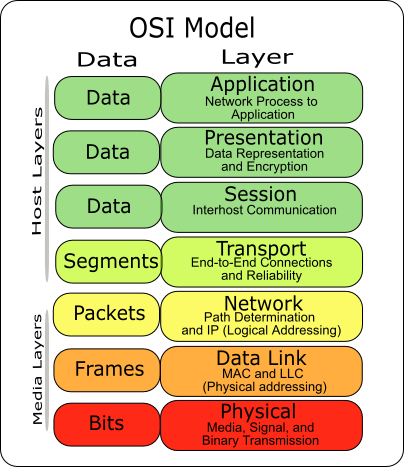
\includegraphics[width=0.4\textwidth,]{fig/Osi-model-jb.png}
	}
	\caption{OSI model} \label{fig: OSI model}
\end{figure*}

\begin{figure*}
	\centering
	{
		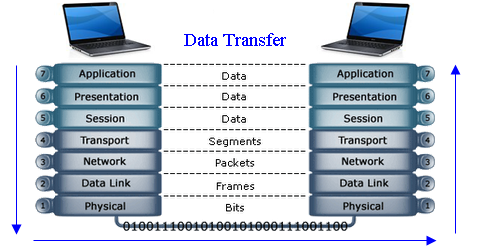
\includegraphics[width=0.6\textwidth,]{fig/osi-model.png}
	}
	\caption{Data Transfer in OSI model} \label{fig: OSI channel}
\end{figure*}

In network terminology, 8 bits is called an OCTET. For the purpose of readability we use the general computer science term BYTE to represent the unit consists of 8 bits.

A combination of protocols at each layer is called a protocol stack, or a protocol suite. The protocol stack until application layer are usually handled by the operating systems. There are several systems specifically aimed to support WSN applications. Contiki\cite{Contiki} is a highly customisable system with 6LoWPAN protocol stack with many hardware supported, OpenWSN\cite{OpenWSN} also has a well hardware support and is featuring full protocol support up to CoAP\cite{rfc7252}, FreeRTOS\cite{FreeRTOS} is optimised for real time tasks, etc.

Due to popularity, in this report we mainly focus on Contiki and the 6LoWPAN protocol stack.

\section{Physical Layer}
Physical Layer specifies the hardware requirements for devices. It defines data transmission at bit level.

WSN features, as explained by its name, wireless connectivity. 802.15.4\cite{802154} standard is supported in many recent WSN devices. Its Physical Layer specification is intended to be for embedded devices emphasising low energy, low cost and low speed. Bluetooth Low Energy\cite{BLE}, BLE, is another candidate for WSN with similar features. \cite{802154BLE} provides a performance analysis of 802.15.4 and BLE.

Usually the length MAC frame, which we explain in \Cref{Sec: Data Link Layer}, is announced before it is being transmitted, e.g. shown in \Cref{Fig: 802.15.4 PHY Frame}.

\begin{table}[h!]
	\centering
	\begin{tabular}{|l|l|l|l|}
		\hline
		Preamble & SFD & MAC frame Length & Reserved \\ \hline
	\end{tabular}
	\caption{802.15.4 PHY Frame}
	\label{Fig: 802.15.4 PHY Frame}
\end{table}

Preamble is used for hardware synchronisation. Start Frame Delimiter is a constantly 0xE5 for 802.15.4 frames. The length of a MAC frame is 0 to 127 bytes. More details can be found in \cite{802154}.

\section{Data Link Layer} \label{Sec: Data Link Layer}
Data Link Layer solves the problem of how the media is controlled. It also defines the atomic data chunk, called frames, being transmitted over the physical channel. Data Link protocols are strongly related to physical features of underlining devices. This layer is sometimes referred as MAC layer and the frame is called MAC frame in many context. MAC protocol only solves single hop communication. Packet forward is defined in upper layer protocols.

With respect to Media Access Control, MAC, technologies such as CSMA/CA \cite{802154} standard and TSCH\cite{TSCH} provides solutions to at which timing and channel should the radio transceiver send and receive data. ContikiMAC\cite{ContikiMAC} proposes a Radio Duty Cycle, RDC, protocol that aims to be energy efficient and has been implemented on Contiki OS.

Another major component in Data Link Layer protocols is the format of different types of frames. In this research, we focus on 802.15.4 standard as its increasing attention in both industry and academy. 

Implementing security measures at this layer is called Link Layer SECurity, LLSEC. 

\subsection{802.15.4 MAC Layer} \label{Subsec: 802.15.4 MAC Layer}

There are four types of frames defined in this standard, which are:
\begin{description}
	\item[\textbf{Beacon}] broadcastes to physically organise the network.
	\item[\textbf{Command}] is used in network maintenance.
	\item[\textbf{Data}] carries actual payload.
	\item[\textbf{ACK}] only optionally sent in response when requested.
\end{description}

Among these types of frames, we are particularly interested in Data frames. We will explain our concern of this choice later in \Cref{Sec: Leakage Sources}. \Cref{Fig: 802154 frame} describes the format of a 802.15.4 Data frame.

\begin{figure*}[h!]
	\centering
	\begin{tabular}{|c|c|c|c|c|}
		\multicolumn{3}{c}{\textit{MAC Header}}                           & \multicolumn{1}{c}{\textit{MAC Payload}} & \multicolumn{1}{c}{\textit{MAC Footer}}     \\ \hline
		2 (bytes)     & 1                    & 4 to 20              & *           & 2              \\ \hline
		Frame Control & Data Sequence Number & Address Information & Data        & Frame Checksum \\ \hline
	\end{tabular}
	\caption{802.15.4 Data Frame}
	\label{Fig: 802154 frame}
\end{figure*}

We briefly explain the format of 802.15.4 Data frame.
\begin{description}[style=nextline]
	\item[\textbf{Frame Control}]
	This 2 bytes field contains the bit flags of additional information that instructs how the receiver should interpret this frame, including the type of this frame, whether the security option is enabled and how the source and destination addresses are represented. When the security option is enabled, additional field will be added to the frame. We will explain the security enabled frame format later in \Cref{Sec: Data Link Layer}. A full explanation of the flags can be found in \cite{802154}.
	
	\item[\textbf{Sequence Number}]
	Each packet is assigned a sequence number. The main purpose of this field is that it enables a simple acknowledgement mechanism, ACK, at MAC layer. Since MAC layer provides only unreliable transmission, i.e. MAC frames are allowed to be dropped or arrive disordered; hence the ACK is optional. However, some other protocol can utilise this ACK, e.g. ContikiMAC uses the ACK MAC frame to inform the sender that the frame is received and hence terminates the resending process of sender.
	
	\item[\textbf{Address Information}]
	This field contains the source address and destination address of this frame. The length of address is variable. Simply speaking, a longer addresses is used for larger network. and shorter for smaller. Each device has a unique built in address as known as MAC address. The MAC address is configurable on some, in fact nearly all recently, devices. Broadcast is achieved by using a specific destination address but group multicast is not implemented on this layer. In fact, given the physical character of radio, both broadcast messages and unicast messages are technically broadcasted. It entirely depends on the receiver to dropping frames that specifies an unicast address of other nodes.
	
	\item[\textbf{Data}]
	This is the MAC layer data. This data is constituted of upper layer protocol headers and application data.
	
	\item[\textbf{Frame Checksum}]
	The checksum is used to check and correct the error induced by physical channel.
\end{description}

The Frame Control, Sequence Number and Address Information together are called MAC header. The Data field is called MAC payload accordingly. 

802.15.4 standard specifies the Maximum Transmission Unit, MTU, to be 127 bytes including the MAC header and footer. That is to say any 802.15.4 compatible hardware must be able to send at least 127 bytes within one frame; any frame that is larger than this size is not guaranteed to be support by the device. Since the MAC header and footer consumes 25 bytes in a Data frame, there is actually 102 bytes left for MAC payload.

Setting the security flag in Frame Control enables 802.15.4 security and adds additional information into the MAC header. We introduce the 802.15.4 security later in \Cref{Subsec: 802154 Sec}.

\subsection{802.15.4 Security} \label{Subsec: 802154 Sec}
802.15.4 security is based on symmetric cryptography, namely Authenticated Encryption with Associated Data, AEAD, scheme. To be more specifically, it provides encryption for MAC payload and authenticity for both MAC header and payload. The cryptographic primitive adopts AES-128 as the block cipher.

802.15.4 has a set of configurable security levels:
\begin{itemize}
\item Encryption only, i.e. only MAC payload is encrypted in CTR mode.
\item Authentication only, i.e. a tag is attached at the end of Data field. The tag is computed on MAC header and MAC payload in CBC mode. The MAC payload is transmitted in plaintext.
\item Encryption and authentication. The whole frame is processed in CCM*\cite{802154} mode, with MAC header being the associated data and MAC payload being the plaintext to be encrypted. The asterisk symbol represents a slight restriction which requires the nonce, or IV, must contain the encoded format specifier that can uniquely determine the format of output ciphertext. In other words, the receiver must can uniquely determine solely by nonce whether authentication and encryption are enabled as well as the length of authentication tag.
\item The tag can be further configured to be 32 bit, 64 bit or 128 bit when authentication is enabled.
\end{itemize}

The format of a 802.15.4 Data frame with security option set is described in \Cref{Fig: 802154 sec frame}.

\begin{figure*}[h!]
	\centering
	\begin{tabular}{|c|c|c|c|c|c|c|}
		\multicolumn{4}{c}{\textit{MAC Header}}                                                             & \multicolumn{2}{c}{\textit{MAC Payload}} & \multicolumn{1}{c}{\textit{MAC Footer}}     \\ \hline
		\multicolumn{3}{|c|}{\multirow{2}{*}{As MAC header in \Cref{Fig: 802154 frame}}} & 0 to 14                    & *             & 0/4/8/16         & 2              \\ \cline{4-7} 
		\multicolumn{3}{|c|}{}                                           & Auxiliary Security Header & Data          & MIC              & Frame Checksum \\ \hline
	\end{tabular}
	\caption{802.15.4 Frame with security option enabled} \label{Fig: 802154 sec frame}
\end{figure*}

The Auxiliary Security Header contains the additional information needed by 802.15.4 security.

\begin{description}[style=nextline]
	\item[\textbf{Security Level}]
	Security Level is represented by the first 3 bits in Auxiliary Security Header. The highest bit controls whether encryption is enabled. The lower two bits controls the length of MIC with the value $0$ indicates no authentication.
	\item[\textbf{Frame Counter}]
	This 4 byte filed increases by one for each frame sent. It is also used for replay detection.
	\item[\textbf{Key Strategy}]
	The other parts instructs which key to be used for this frame. The keys are presumed to be pre-shared in PAN Information Base, PIB, which is a database containing information that is shared among the network. Keys are managed by groups and indexes within a group. The definition of groups depends on upper layer applications.
\end{description}

More details of Auxiliary Security Header is defined in the 802.15.4 standard.

Message Integrity Code, MIC, is equivalent to the cryptography term Message Authenticate Code, MAC. Therefore the term MIC is used to avoid confusion with Media Access Control.

Access Control List, ACL, is a list data structure defined in 802.15.4. It is used to maintain 802.15.4 security access during runtime.Each entry in ACL is paired with another node.  An ACL entry contains the following elements:
\begin{description}
	\item[\textbf{Address}] The address of remote node, used as an identifier.
	\item[\textbf{Security Suite}] The security level to use associated to the address.
	\item[\textbf{Key}] The paired cryptographic key associated to the address.
	\item[\textbf{Last Initial Vector}] Nonce used for the last outgoing frame.
	\item[\textbf{Replay Counter}] Nonce received for the last incoming frame.
\end{description}
On sending a frame with security option, the sender looks up destination address in ACL and determines the security level, key and frame counter which is encoded into the last initial vector. On receiving a frame, the receiver looks up source address in ACL and checks for match of the security suite and security level in the frame. Then it verifies the frame with the key. If replay protection is enabled, the replay counter is also compared. Failing any of the tests will result into rejecting of the frame.

\subsection{Nonce of CCM* in 802.15.4 security}
As stated earlier in \Cref{Subsec: 802154 Sec}, CCM* requires that the format of ciphertext can be uniquely deduced from the nonce. \Cref{Fig: CCM nonce} describes the nonce used for encryption.

\begin{figure*}[h!]
	\centering
	\begin{tabular}{|c|c|c|c|c|}
		\hline 
		1 (bytes) & 8              & 4             & 1              & 2             \\ \hline
		Flag      & Source Address & Frame Counter & Security Level & Block Counter \\ \hline
	\end{tabular}
	\caption{CCM* nonce for encryption}
	\label{Fig: CCM nonce}
\end{figure*}

\begin{description}
\item[\textbf{Flag}]
This is a constant a value equals to 0x02.
\item[\textbf{Source Address}]
This field is the address of sender. If an address of length than 8 byte is used, it will be extended to 8 byte.
\item[\textbf{Frame Counter}]
The frame counter is directly mapped from the same filed in Auxiliary Security Header, as described earlier.
\item[\textbf{Security Level}]
As of frame counter, security level is also directly mapped from Auxiliary Security Header with the highest bit set to $0$. As described earlier, security level solely determines the format of ciphertext.
\item[\textbf{Block Counter}]
This is exactly the block index of MAC payload, increases by one for each block. Since AES-128 is the underlining block cipher; therefore the block size is 128 bit.
\end{description}

802.15.4 security could either be implemented by hardware and/or software. Some platform may not support the security option, or only supports a sub set of this measure. We briefly describe an implementation on Contiki platform later in \Cref{Subsec: noncoresec}.

\subsubsection{Implementation on Contiki: noncoresec} \label{Subsec: noncoresec}
noncoresec is the LLSEC implementation on Contiki. It is a reduced implementation of 802.15.4 security which supports only a network shared key hard coded into the kernel code.

\subsection{Sub Layer: RDC Layer}
In practical, the radio transceiver turned out to be the most energy consuming part in a sensor node. Further more, listening data consumes more energy than sending them. Thus an optimisation for energy preserving is to switch off the transceiver for most of the time and switch it on only when there is data on air. The Radio Duty Cycle, RDC, Sub Layer is therefore added to MAC Layer. RDC protocols control the behaviour of radio transceiver by synchronise their timing of sending and receiving data; hence the radio can be kept off for most of the time. In the case of Contiki, there are two RDC protocols implemented:
\begin{itemize}
\item \textbf{nullrdc}. There is no RDC protocol. The transceiver is kept on forever.
\item \textbf{ContikiMAC\cite{ContikiMAC}}. The transceiver is kept off for most of the time and only wakes up for a short period. If data transmission is detected during the wake-up period, the receiver keeps the transceiver on until the frame is received and informs the sender with an ACK. On the other hand, the sender continuously retransmits the frame until an ACK is received or the time runs out.
\end{itemize}

Time-Slotted Channel Hopping\cite{TSCH}, TSCH, is another RDC protocol that is adopted by OpenWSN. Since it is not implemented yet in our platform, Contiki, we omit its further details in this report.

\section{Network Layer}
The Data Link Layer protocol has solved the problem of data transmission over directly linked nodes. However, real world WSN applications are sometimes deployed in a wider range that not all nodes can be directly connected, such as a smart city application. The solution to build a logic data path between the nodes where each intermediate node forwards the data to the next node until it reaches its destination. Such logical data path is called a multi hop connection and directly connected data path is called a single hop connection respectively. The transmission unit at the Network Layer is called a packet.

A network is defined as a set of nodes logically connected to each other. There are two common types of network considered in WSN applications:
\begin{description}[style=nextline]
	\item[\textbf{Star Network}]
	Star network is a centralised network, as in \Cref{fig: Star Network}. Each node is directly linked to the centre. Star networks can be easily implemented and thus requires less resources.
	\item[\textbf{Mesh Network}]
	Mesh network has a decentralised structure as shown in \Cref{fig: Mesh Network}. Every node is capable to forward packets. Comparing to star network, mesh network is more flexible and scalable but also more complicate and harder to implement. Mesh network is more practical than star network in large scale applications, such as smart cities.
\end{description}

\begin{figure*}
	\centering
	\begin{subfigure}[b]{0.5\textwidth}
		{
			
\includegraphics[width=0.5\textwidth,]{fig/StarNetwork.png}
		}
		\subcaption{Star Network} \label{fig: Star Network}
	\end{subfigure}
	\begin{subfigure}[b]{0.5\textwidth}
		{
			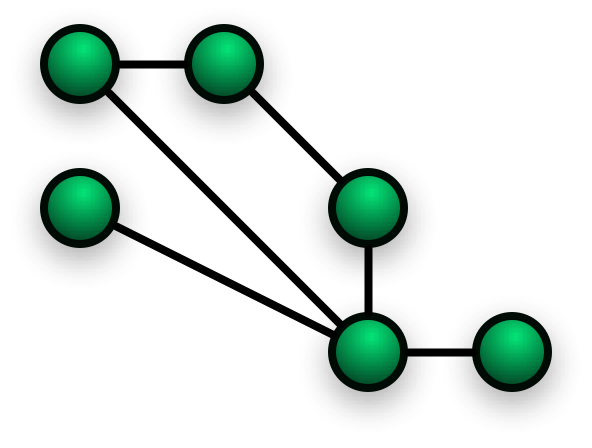
\includegraphics[width=0.5\textwidth,]{fig/NetworkTopology-Mesh.png}
		}
		\subcaption{Mesh Network} \label{fig: Mesh Network}
	\end{subfigure}
	\caption{Network Topologies} \label{fig: Network topologies}
\end{figure*}

Some network are built with a hybrid approach of star network and mesh network, e.g. the Cluster Tree Network of Zigbee\cite{Zigbee} as showed in \Cref{fig: ZigBee Topologies}.

\begin{figure*}[h!]
	\centering
	{
		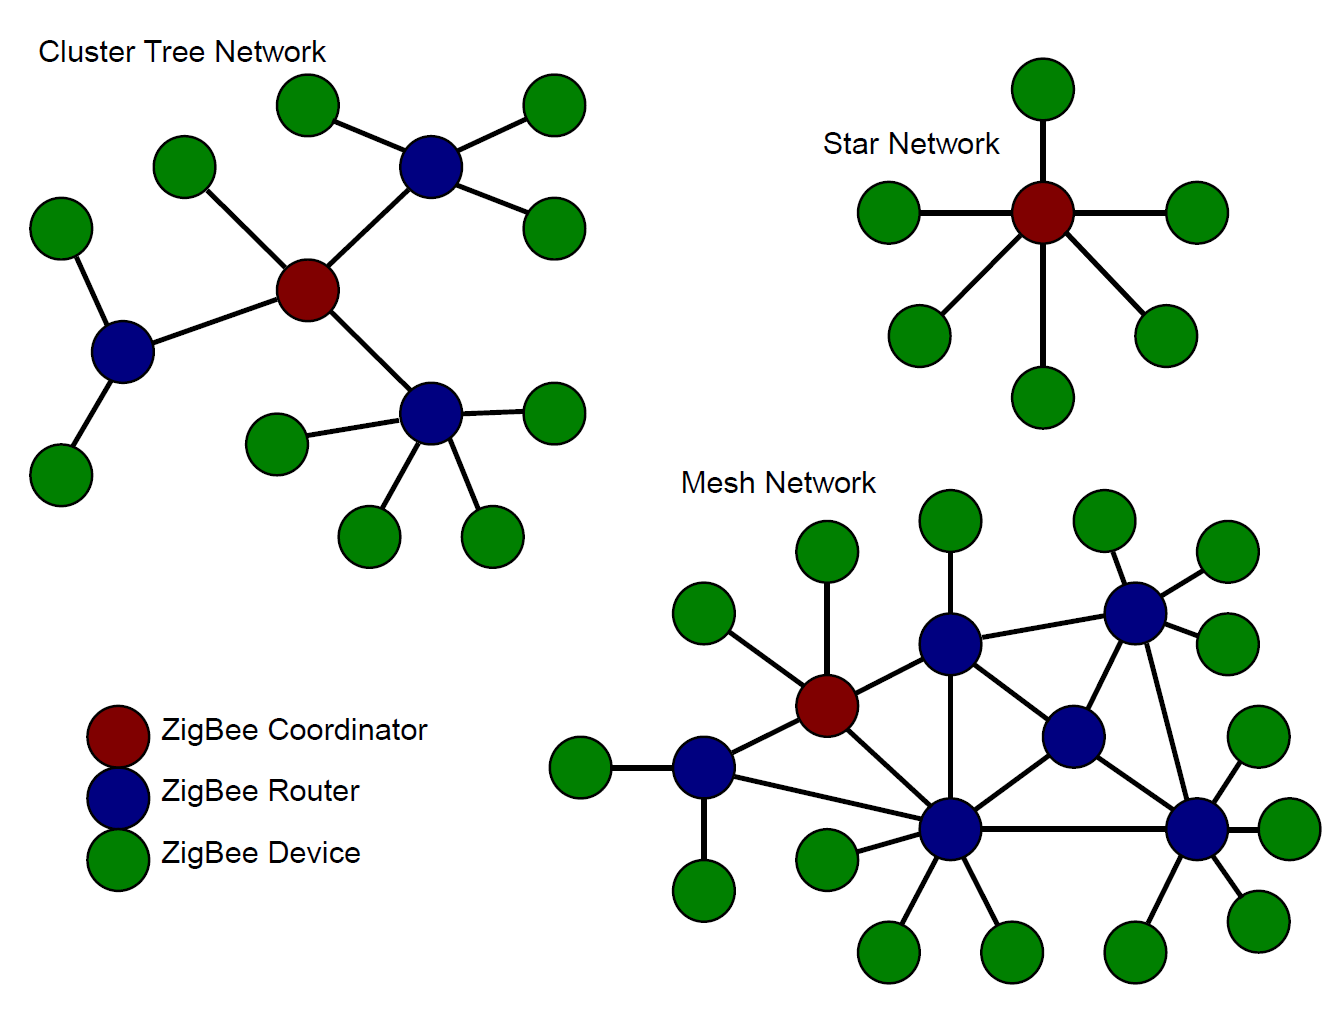
\includegraphics[width=0.7\textwidth,]{fig/ZigBeeTopologies.png}
	}
	\caption{Different ZigBee Network Topologies} \label{fig: ZigBee Topologies}
\end{figure*}

6LoWPAN is a currently well adopted network standard. It has the following features making it popular in IoT industry: 
\begin{itemize}
	\item Each device is assigned with an IPv6 address of compressed format. With a border router that translates the compressed IPv6 address into an IP address, a node inside 6LoWPAN  can directly communicate with a host over Internet.
	\item Its mesh routing feature lead to a flexible, scalable and robust network, as the network can spontaneously reorganise itself at running time.
	\item It is standardised by IETF and well supported in industry.
\end{itemize}

As of this project, we are particularly interested into 6LoWPAN due to the reasons above. Packets in a 6LoWPAN can be categorised into two classes:
\begin{enumerate}
	\item \textbf{IPv6 Data Packets}
	\item \textbf{ICMPv6 Packets}
\end{enumerate}
We give a brief explanation of their contents in \Cref{Subsec: IPv6 Data Packets} and \Cref{Subsec: ICMPv6} respectively.

\subsection{6LoWPAN Adaptation Sub Layer} \label{Subsec:6LoWPAN Adaptation Sub Layer}
A sub layer is defined in 6LoWPAN standard\cite{rfc4944} to compress a standard IPv6 header, in order to reduce the overhead induced by protocol stacks and provide more bandwidth to the applications. Additional headers are prepended before the IPv6 header as shown in \Cref{Fig: 6LoWPAN Adaptation Header}. 

\begin{figure*}[h!]
	\centering
	\begin{tabular}{|l|l|l|}
		\hline
		6LoWPAN Adaptation Header & Compressed IPv6 Header & IPv6 Payload \\ \hline
	\end{tabular}
	\caption{6LoWPAN Adaptation Header}
\label{Fig: 6LoWPAN Adaptation Header}
\end{figure*}

The header compression is generally done by:
\begin{itemize}
	\item Optimised encoding. Take the Hop Limit, HLIM or TTL (Time To Live), field for example, the frequently used values, 1, 64 and 255, are represented in 2 bits as 01b, 10b and 11b respectively, saving 6 bits from its original 1 byte field.
	\item Since 6LoWPAN has usually less devices than a normal IPv6 network. The unused higher bits are therefore re-encoded. Technically speaking this is also a kind of optimised encoding.
\end{itemize}
The header compression is a lossless; thus we can always reconstruct an equivalent IPv6 header from the compressed header and this header compression information. We omitted further complicated details due to its complexity but they are defined in \cite{rfc6282}.

In addition to header compression, 6LoWPAN Adaptation Header also contains information for packet fragmentation as well as device address conflict avoiding. We omit the further details as it is beyond the scope of this report. Details of these mechanisms are defined in \cite{rfc4944}.

\subsection{IPv6 Data Packets} \label{Subsec: IPv6 Data Packets}
These packets contains the IPv6 payload. In 6LoWPAN, the IPv6 header is compressed as described in \Cref{Subsec:6LoWPAN Adaptation Sub Layer}. In this section we explain the contents of a standard IPv6 header instead of a compressed one for convenience but one can always uniquely transform a standard IPv6 header to a compressed one since they are indeed equivalent.

IPv6 is defined in \cite{rfc2460}. Its basic format is as shown in \Cref{Fig: IPv6 Packet Format}. We removed the length information as they are inconsistent when the header is compressed.

\begin{figure*}[h!]
\center
	\begin{tabular}{l|c|c|c|c|c|c|}
	\cline{2-7}
	\multirow{2}{*}{\textit{IP Header}} & Version & Traffic Class & Flow Label & Payload Length & Next Header & Hop Limit \\ \cline{2-7} 
	                                & \multicolumn{3}{c|}{Source Address}  & \multicolumn{3}{c|}{Destination Address} \\ \cline{2-7} 
	\textit{IP Payload}                 & \multicolumn{6}{c|}{Payload}                                                    \\ \cline{2-7} 
	\end{tabular}
	\caption{Basic IPv6 Packet Format} \label{Fig: IPv6 Packet Format}
\end{figure*}

\begin{description}[style=nextline]
	\item[\textbf{Version}]
	In 6LoWPAN this is constant 0x6.
	\item[\textbf{Traffic Class}]
	This field is default by 0 and may be set by an upper layer application as a hint of packet. A router can act accordingly to this field, such as adjusting the priority of packet, or even modify this value upon forward. The support for values other than $0$ is optional.
	\item[\textbf{Flow Label}]
	This field is intended to label a logical data path at Network Layer. The IPv6 standard\cite{rfc2460} states  it should ``be used by a source to label sequences of packets for which it requests special handling by the IPv6 routers, such as non-default quality of service or `real-time` service``. Support to this field is optional.
	\item[\textbf{Payload Length}]
	This field specifies the length of Network Layer payload.
	\item[\textbf{Next Header}]
	This field specifies the Transportation Layer protocol to be used. In WSN applications this is usually UDP. We will cover more of this in \Cref{Sec: Transportation Layer}.
	\item[\textbf{Hop Limit}]
	Hop Limit, HLIM, is also called Time To Live, TTL. It decreases by one whenever the packet is forwarded. The packet will be dropped when this value reaches $0$. This prevents a packet from being infinitely forwarded.
	\item[\textbf{Source Address and Destination Address}]
	These are the IPv6 addresses of sender and receiver. These are addresses are normally consistent during routing of a packet. In comparison,MAC source and destination varies on each hop, as an intermediate receiver becomes the sender of next hop.
	\item[\textbf{Payload}]
	This field contains the upper layer protocol headers and application data.
\end{description}
One thing to be noticed is that Traffic Class and Flow Label is not yet fully defined by IPv6 standard.

There are also extension headers defined in IPv6\cite{rfc2460}, including IPsec and fragmentation ,etc.

IPsec is defined in \cite{rfc4301} with its Authentication Header, AH, defined by \cite{rfc4302} and Encapsulating Security Payload, ESP, defined by \cite{rfc4303}. AH authenticates all IP Headers (the basic IPv6 header and the extensions) except fields  those might be modified by a router such as TTL. ESP provides encryption over IP Payload. Enabling IPsec over IPv6 adds 40 bytes to the IP Header which is unacceptable in IoT environment. \cite{6LoWPANIPsec} and \cite{CompressIPsec} discusses compression of IPsec over 6LoWPAN. \cite{ContikiIPsec} describes an implementation of IPsec over Contiki but it is not yet adopted by the latest released Contiki 3.0.

We omit further details of other extension headers as they are mostly used to handle routing and fragmentation and thus beyond the scope of this report.

\subsection{ICMPv6 Packets} \label{Subsec: ICMPv6}
Internet Control Message Protocol for IPv6, ICMPv6, is a set of messages that are used to maintain the network. \cite{rfc4443} defines the general format alongside with ICMPv6 Error Messages and Information Messages. 

%IPv6 General Format
In IPv6, an ICMP messages is preceded by an IPv6 Basic Header and optional IPv6 extension headers with the last Next Header field set to ICMP as \Cref{Fig: ICMP with IPv6}. The IP Payload in \Cref{Fig: IPv6 Packet Format} is replaced by an ICMP message in this case.

\begin{figure*}[h!]
	\centering
	\begin{tabular}{|l|l|l|}
		\hline
		IPv6 Basic Header & Extension Headers (optional) & ICMP Message \\ \hline
	\end{tabular}
	\caption{ICMP Message with IPv6 Headers}
	\label{Fig: ICMP with IPv6}
\end{figure*}

The general format of an IPv6 message is described in \cite{rfc4443} as \Cref{Fig: General Format of ICMPv6 Message}.
\begin{figure*}[h!]
	\centering
	\begin{tabular}{|c|c|c|c|}
	\hline
	1 (byte) & 1    & 2        & *            \\ \hline
	Type     & Code & Checksum & Message Body \\ \hline
	\end{tabular}
	\caption{General Format of ICMPv6 Message}
	\label{Fig: General Format of ICMPv6 Message}
\end{figure*}

As stated in \cite{rfc4443},
\begin{description}[style=nextline]
\item[\textbf{Type}]
There are two groups of types of messages defined in \cite{rfc4443}. Error messages have a Type value in $[0,127]$ which indicates an error of network. Information messages have a type value in $[128,255]$ which provide network information to nodes of the network.
\item[\textbf{Code}]
Each type of ICMP message defines its own code to indicate the exact functionality of an ICMP message.
\item[\textbf{Checksum}]
Checksum for the packet.
\end{description}

We explain only a minor set of ICMP Messages that we have successfully observed in our experiment.
%Error messages, informative message
\begin{description}[style=nextline]
\item[\textbf{Echo Request and Reply Messages}]
These are diagnostic ICMP Information messages. Upon receiving an ICMP Echo Request, the receiving node is required by \cite{rfc4443} to reply with an identical ICMP message except the source and destination addresses are inverted. The Echo Request is typically sent by a PING command for diagnostic reasons such as testing of connectivity or measuring the Round Trip Time, RTT, of a data path. The response of ICMP Echo is enabled in Contiki by default but it is disabled on many Internet server for security reasons.
\end{description}

%RPL messages
A family of ICMPv6 messages, RPL messages, are defined by \cite{rfc6550}. RPL messages are fundamental in forming and self-organising a 6LoWPAN network. A 6LoWPAN network instance is a Destination Oriented Directed Acyclic Graph, DODAG, shown in \Cref{Fig: DODAG}. 
\begin{figure*}[h!]
	\center
	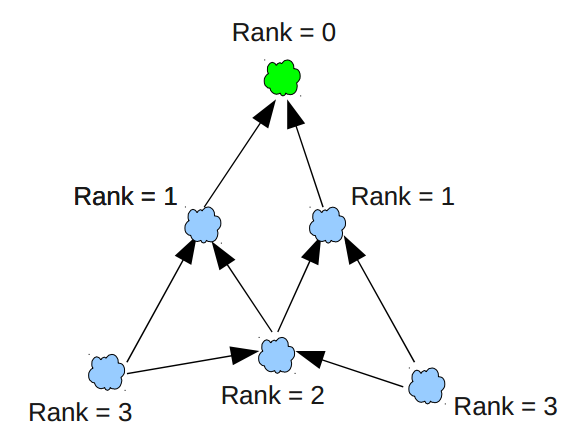
\includegraphics[width=0.6\textwidth]{fig/dodag.png}
	\caption{A DODAG}
	\label{Fig: DODAG}
\end{figure*}
We omit further details of the decision of a routing path as it is beyond the scope of this report but they are defined in \cite{rfc6550}. Instead, we explain the major related ICMP messages in a 6LoWPAN network.
%DODAG Information Solicitation
%DODAG Information Object
%Destination Advertisement Object
\begin{description}[style=nextline]
\item[\textbf{DAG Information Object (DIO) Message}]
The DIO message contains the global information of a 6LoWPAN network. It is broadcasted by a node to its neighbours periodically for maintenance, or as a reply on request of a new joining node to provide enough information for the new one to join the network.

\item[\textbf{DAG Information Solicitation (DIS) Message}]
When a new node is booted, it broadcasts DIS messages probing an existing 6LoWPAN network. If the DIS message is received by any neighbour node that belong to a network, then a DIO message is replied providing the information to join the network.

\item[\textbf{Destination Advertisement Object (DAO) Message}]
DAO Message is sent by a child node to its precedents to propagate its routing information. The routing information is later used when another node tries to send a packet to this child node. The receiving parent can either store the routing information or forward it to an upper level parent depending on its capability.
\end{description}

\cite{rfc6550} also defined secure variants to these RPL messages which provides authentication as well as confidentiality. However, they are not implemented on our platform and therefore we omit their details in this report.

\section{Transport Layer} \label{Sec: Transportation Layer}
Transport Layer defines the interface to applications. To be more specifically, ports are defined at this layer in addition to network addresses allowing packets to be directed to different applications running on the same host. Transport Layer protocols also define more semantic details of the data channel, such as reliability and modes data operation.

TCP and UDP are the most widely used Transport Layer protocols over Internet. TCP provides a reliable streamed data channel whilst UDP provides only unreliable datagrams. In the world of IoT, UDP is generally preferable due to its low overhead and support to multicast.

\subsection{UDP}
UDP is defined by \cite{rfc768}. Its format is shown in \Cref{Fig: UDP Datagram Format}
\begin{figure*}[h!]
	\center
	\begin{tabular}{ccccc}
		\multicolumn{4}{c}{\textit{UDP Header}}                                                                                                                & \textit{UDP Payload}         \\ \hline
		\multicolumn{1}{|c|}{\textit{2 (bytes)}} & \multicolumn{1}{c|}{2}                & \multicolumn{1}{c|}{2}              & \multicolumn{1}{c|}{2}        & \multicolumn{1}{c|}{*}       \\ \hline
		\multicolumn{1}{|c|}{Source Port}        & \multicolumn{1}{c|}{Destination Port} & \multicolumn{1}{c|}{Payload Length} & \multicolumn{1}{c|}{Checksum} & \multicolumn{1}{c|}{Payload} \\ \hline
	\end{tabular}
	\caption{UDP Datagram Format}
	\label{Fig: UDP Datagram Format}
\end{figure*}

\begin{description}[style=nextline]
	\item[\textbf{Source and Destination Port}]
	Ports are the identifier of applications running on a host. The source port and destination port semantically represent the applications that send and receive the data respectively.
	\item[\textbf{Payload Length}]
	The length of UDP payload.
	\item[\textbf{Checksum}]
	Checksum of the packet. The checksum is optional in \cite{rfc768} but is required in 6LoWPAN.
	\item[\textbf{Payload}]
	The application data.
\end{description}

The UDP header constitutes of 8 bytes and contains only the minimum information for the OS to identify the receiving process of a packet. Data transmission of UDP is unreliable, which means the data might be lost or arrive disordered.

The combination of a network address and a port is called an entity in network term.

\section{Application Layer}
%DTLS
%MQTT
%CoAP
This layer represents the various applications on the architecture. Some Application Layer protocols may beneath other applications, such as TLS and DTLS are sometimes viewed as a sub layer protocol of Transport Layer.

In this section we describe two typical Application Layer protocols that has been implemented on our platform, namely DTLS\cite{rfc6347} and CoAP\cite{rfc7252}. A real application can be built on these protocols.

\subsection{DTLS}
DTLS\cite{rfc6347} stands for Datagram Transport Layer Security. As of TLS, it provides end-to-end data confidentiality and authenticity. The main difference between DTLS and TLS is that:
\begin{itemize}
	\item DTLS is built on datagrams instead of TCP like TLS. In case of a 6LoWPAN network, this is effectively UDP. As a result DTLS implemented a simple reliable transmission mechanism during handshake to reliably exchange the cryptographic materials.
	\item Explicit sequence number and epoch values on each DTLS record. We explain theses values in following context.
	\item Invalid records no longer terminate the connection. Instead, errors are suppressed to the upper layer application and an alert is sent.
	\item RC4 is disabled due to its stateful design\cite{DtlsCiphers}. It is hard to maintain synchronised stated with UDP.
\end{itemize}

A packet containing Application Layer data is called a record. The format of a DTLS record is as depicted in \Cref{Fig: DTLS Record Format}.
\begin{figure*}[h!]
	\center
	\begin{tabular}{cccccc}
		\multicolumn{5}{c}{\textit{DTLS Header}}                                                                                                                                     & \textit{DTLS Encrypted Payload} \\ \hline
		\multicolumn{1}{|c|}{1 (byte)}     & \multicolumn{1}{c|}{2}                & \multicolumn{1}{c|}{2}     & \multicolumn{1}{c|}{6}               & \multicolumn{1}{c|}{2}      & \multicolumn{1}{c|}{*}          \\ \hline
		\multicolumn{1}{|c|}{Content Type} & \multicolumn{1}{c|}{Protocol Version} & \multicolumn{1}{c|}{Epoch} & \multicolumn{1}{c|}{Sequence Number} & \multicolumn{1}{c|}{Length} & \multicolumn{1}{c|}{Fragment}   \\ \hline
	\end{tabular}
	\caption{DTLS Record Format}
	\label{Fig: DTLS Record Format}
\end{figure*}

\begin{description}[style=nextline]
	\item[\textbf{Content Type}]
	Content Type is inherited from TLS. It indicates the type of this record. The value can either be:
	\begin{enumerate}
		\item CHANGE\_CIPHER\_SPEC($20$)
		\item ALERT($21$)
		\item HANDSHAKE($22$)
		\item APPLICATION\_DATA($23$)
	\end{enumerate}
	In the case of CHANGE\_CIPHER\_SPEC and HANDSHAKE, the sub protocols are invoked accordingly. Otherwise the Fragment field is treated as an error code in case of ALERT or ciphertext of application data in case of APPLICATION\_DATA.
	\item[\textbf{Protocol Version}]
	DTLS uses the complement of \{0xff, 0xff\} to indicate the version number. Since the implementation on our platform is for DTLS 1.2, this field is constantly \{0xfe, 0xfd\}.
	\item[\textbf{Epoch}]
	This field is incremented by one for each cipher state change, such as an invocation of \\
	CHANGE\_CIPHER\_SPEC. This value is used as an index of which set of cryptographic materials to be used, such as algorithms, keys or nonces.
	\item[\textbf{Sequence Number}]
	This field is the sequence number of this record. The sequence number is used by some cryptographic algorithms, such as to form a part of nonce.
	\item[\textbf{Length}]
	The length of Fragment field.
	\item[\textbf{Fragment}]
	The content of Fragment depends on Content Type. In the case of APPLICATION\_DATA, the Fragment contains the ciphertext.
\end{description}

The DTLS on Contiki is implemented by a third party code, tinydtls-0.8.2\cite{tinydtls}. Its current version supports two ciphersuites, namely:
\begin{itemize}
	\item TLS\_ECDHE\_ECDSA\_WITH\_AES\_128\_CCM\_8\cite{rfc7251}
	\item TLS\_PSK\_WITH\_AES\_128\_CCM\_8\cite{rfc6655}
\end{itemize}
Both ciphersuites adopts the same AEAD scheme, AES\_128 with CCM mode, as their cryptographic primitives. Further details of the AEAD scheme is defined in \cite{rfc5116} and \cite{CCM}.

One thing to be noticed is that DTLS is not compatible with the multicast feature of IPv6 and UDP. The direct reason is the distribution of cryptographic materials poses a great difficulty in IoT applications. \cite{DtlsMulticast1} and \cite{DtlsMulticast2} discuss this topic in further details.

As of this project, we are mostly focused on the APPLICATION\_DATA records rather than the handshake process, as we consider the later to be performed independently from any upper layer application.

\subsection{CoAP}
Constrained Application Protocol, CoAP, is a general application data interface defined in \cite{rfc7252}. CoAP can be viewed as a variation of HTTP that is specifically designed to access resources on IoT devices. The high level concept of CoAP is to make accessing data on sensor nodes behaves as accessing resources of a web site on Internet. Generally speaking,
\begin{itemize}
	\item Typically the sensor node runs a CoAP server application and registers its resources (sensors, actuators) to CoAP server. The management node, operated by an user or higher level application, access the resources as a CoAP client. In some cases the sensor node can also be a CoAP client and requests operational information from the management node which in this case runs as a CoAP server.
	\item Similar to HTTP, CoAP uses a Request-Response application model. That is, the CoAP client actively sends Requests to CoAP server, the CoAP server passively replies to each Request with a Response.
\end{itemize}

We show an example of the execution of CoAP protocol in \Cref{Fig: An Example of CoAP}.
\begin{figure*}[h!]
	\center
	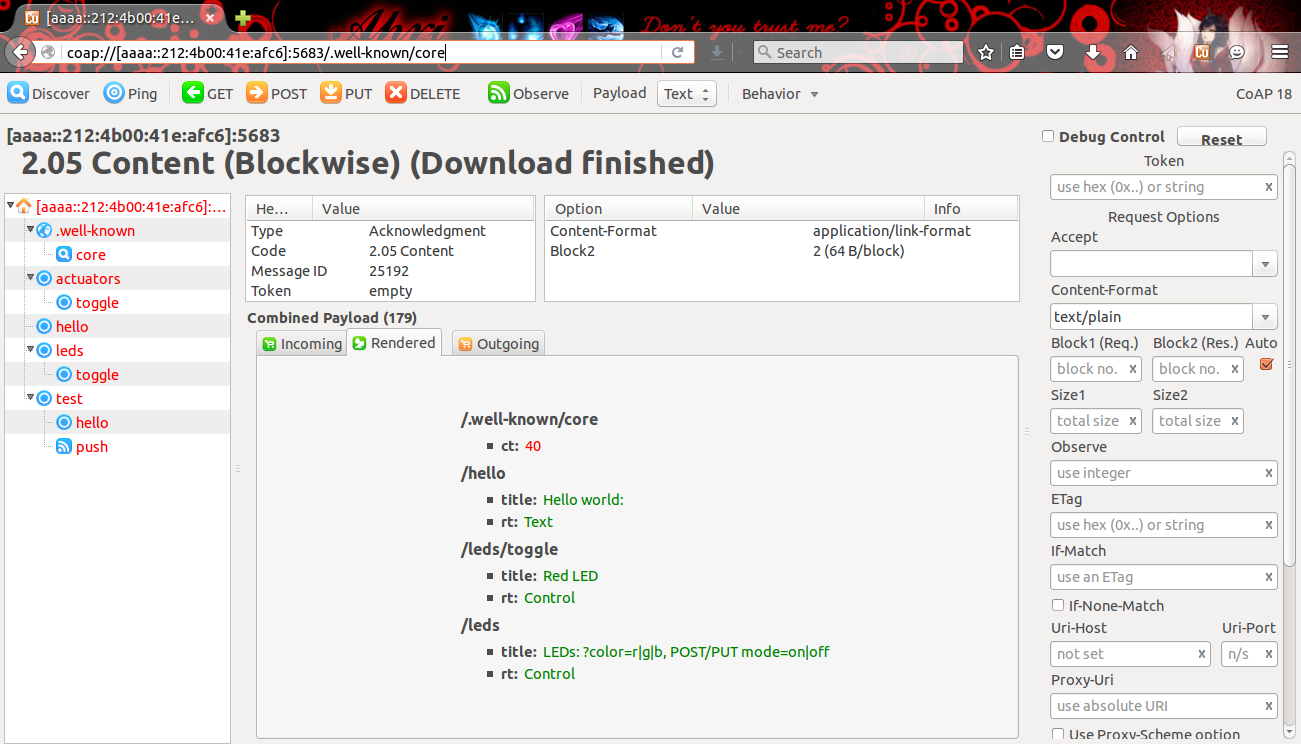
\includegraphics[width=1\textwidth]{fig/CoapExample.png}
	\caption{An Example of CoAP}
	\label{Fig: An Example of CoAP}
\end{figure*}

In the example of \Cref{Fig: An Example of CoAP}, the CoAP server is a CC2538 node registered with several resources, ‘’actuators’’, ‘’hello’’ and ‘’leds’’, etc. The CoAP client is a desktop accessing the data on the sensor node through the Copper plugin\cite{Copper} of Firefox. As shown in \Cref{Fig: An Example of CoAP}, CoAP has the following features:
\begin{itemize}
	\item A node in the 6LoWPAN network is represented by an URL. In \Cref{Fig: An Example of CoAP}, we can see at the address bar the resources of node is represented in a form of URL:\\
	\url{coap://[aaaa::212:4b00:41e:afc6]:5683/.well-known/core} \\
	This is exactly as the same format of those URLs on Internet: \\
	 \{PROTOCOL :// ADDRESS : PORT / LOCATION \}.
	 \item Resources available on the node is organised in a tree structure, as shown in the tree view on the left in \Cref{Fig: An Example of CoAP}. These resources can be specified by the URL as shown in the address bar.
	 \item Similar to HTTP, four methods, namely GET, POST, PUT and DELETE, are defined to access and manipulate the resources on sensor nodes. In addition, a new new option OBSERVE is also defined for GET method which allows a CoAP server to actively push data to the CoAP client. We explain more details of these methods later in the context.
\end{itemize}
%CoAP as TCP
In addition to the definition of general application data interface, CoAP also provides a lightweight reliable transmission mechanism (described later in the context) as well as a fragmentation mechanism\cite{CoapBlock}; therefore some context consider CoAP as a Transport Layer protocol that is an alternative of TCP. For example, \cite{CoDTLS} proposes to use CoAP to perform the DTLS handshake instead of the built in retransmission mechanism of DTLS. CoAP also supports multicast messages as it is based on UDP, comparing to HTTP which is generally based on TCP and supports only one to one communication.
%CoAP format
\Cref{Fig: CoAP Message Format} describes the format of a CoAP message. The Token and Options adopt a length-value representation and thus their lengths are variable. The length of Payload is not explicitly stated but is calculated from the upper layer length.
\begin{figure*}[h!]
	\center
	\begin{tabular}{|c|c|c|c|c|c|c|c|c|}
	\hline
	2 bits  & 2 bits & 4 bits       & 1 byte & 2 bytes   & * & *       & 1 byte    & *       \\ \hline
	Version & Type   & Token Length & Code   & Message ID & Token                 & Options & Payload Marker & Payload \\ \hline
	\end{tabular}
	\caption{CoAP Message Format}
	\label{Fig: CoAP Message Format}
\end{figure*}

\begin{description}[style=nextline]
	\item[\textbf{Version}]
	This is the version of CoAP. Currently this is constantly 0x01.
	\item[\textbf{Type}]
	Type field contains the transmission related information. There are four values defined:
	\begin{itemize}
		\item \textbf{Confirmable(0)}: The message must be confirmed by an acknowledgement, otherwise the sender will attempt to retransmit the message.
		\item \textbf{Non confirmable(1)}: The message does not need to be confirmed and thus the transmission is unreliable.
		\item \textbf{Acknowledgement(2)}: This value is set to confirm the reception of a Confirmable(0) message. Piggyback, i.e. application data sent together within same message, is allowed in CoAP acknowledgement.
		\item \textbf{Reset(3)}: This value is similar to the RST flag in TCP which usually indicates a fatal error in connection and no further message should be sent on the same connection.
	\end{itemize}
	\item[\textbf{Token Length}]
	This field indicates the length of Token field. We explain Token field in the following context.
	\item[\textbf{Code}]
	Code indicates the class of content. The higher 3 bits indicates the class of this message:
	\begin{itemize}
		\item \textbf{Request(0)}: Sent by client requesting access of data of server.
		\item \textbf{Success Response(2)}: A Response by server indicates a successful Request.
		\item \textbf{Client Error Response(4)}: A Response by server indicates an error in the Request. This can be resulted from syntax error in Request or the serve is not capable to process the Request.
		\item \textbf{Server Error Response(5)}: A Response by server indicates an error happened in the server. In this case, the Request is valid such but the server failed due to some internal error.
	\end{itemize}
	The lower 5 bits indicates further details of the code.
	If the message is a Request, these bits indicates the method in the Request:
	\begin{itemize}
		\item \textbf{GET}: The client requests to read the specified resources. Specifically when the OBSERVE option is set for a GET request, the resources can be pushed to the client  without further Requests\cite{rfc7641}.
		\item \textbf{PUT}: The client requests to write the specified resources to a value provided by the client.
		\item \textbf{POST}: The client requests to update the specified resources by a value provided by the client.
		\item \textbf{DELETE}: The client requests to remove data of the specified resources.
	\end{itemize}
	By definition, GET, PUT and DELETE are idempotent, i.e. execution of the Request is stateless. However, the definitions above are only semantic and are not mandatory. Implementations of higher level application could still violate the definitions, such as modifying the data on GET Request.
	
	In case of a Response, the lower bits inherited the error codes in HTTP, as defined in \cite{rfc2616}.
	\item[\textbf{Message ID}]
	Message ID is the index of a message. It is mostly used in reliable transmission to match an acknowledgement with its original message.
	\item[\textbf{Token}]
	Token is an index for a Request-Response session. A Response is matched to a Request with Token. Notice that Message ID and Token are different indexes, since same Token might be reused for multiple messages due to fragmentations, or OBSERVE option, etc.
	\item[\textbf{Options}]
	Options are the arguments for a message, such as URI, content format and size, etc. Different Options are defined for each Request and Response. The full list of Options is defined in \cite{rfc7252}.
	\item[\textbf{Payload Mark}]
	Payload Marker marks the end of Options and any data followed should be treated as Payload.
	\item[\textbf{Payload}]
	This is the application data contained in this message. The content of this field varies according to Code and higher level application.
\end{description}

Based on the similarity between CoAP and HTTP, a CoAP message can be easily translated between its HTTP counterpart by a Cross-Protocol Proxy, as depicted in \cite{rfc7252}.

Erbium\cite{Erbium} project is the CoAP implementation on Contiki, described in \cite{ContikiCoap}. It implements the CoAP engine and defined an interface for developers to implement their own application over the framework. Simply speaking, what developers need to do to integrate their own code into the CoAP framework is simply register their own callback function to the CoAP engine to handle the Requests to different resources.

\subsection{CoAPs}
CoAPs is the security version of CoAP which is the counterpart of HTTPS to HTTP. CoAPs adopts DTLS as the security measure and the any CoAP message should be encrypted as DTLS payload when using CoAPs. CoAPs is defined by \cite{rfc7252} as shown in \Cref{Fig: CoAPs Message}.

\begin{figure*}[h!]
	\center
	\begin{tabular}{cc}
		\textit{}                                  & \textit{DTLS Encrypted Payload}            \\ \hline
		\multicolumn{1}{|c|}{\textit{DTLS Header}} & \multicolumn{1}{c|}{CoAP Message} \\ \hline
	\end{tabular}
	\caption{CoAPs Message}
	\label{Fig: CoAPs Message}
\end{figure*}

The current version of DTLS does not support the multicast feature of CoAP. The multicast alternation of DTLS proposed by \cite{DtlsMulticast1} and \cite{DtlsMulticast2} could be used to adapt CoAPs to multicast messages.

\cite{Lithe} proposes an integration of CoAP and DTLS with compressed headers. Unfortunately we have failed to adapt its source code to our platform as it is implemented on an earlier Contiki version that does not support our device. We have yet found any valid CoAPs implementation on our platform as well.

\section{RIME Stack}
RIME Stack\cite{RIME} is a non-layered WSN communication framework proposed alongside with earlier version of Contiki. Instead of dividing communication between nodes in a layered structure as the OSI model does, RIME Stack organises the communications of WSN in a way such that:
\begin{itemize}
	\item Each node is identified by a RIME address. In practice, the RIME address is directly derived from the hardware address.
	\item RIME Stack defines a set of abstracted communication primitives that can be directly invoked by the applications as well as a set of arguments that controls the connection.
	\item The Chameleon architecture\cite{RIME} acts as an intermediate virtualisation layer that translates RIME Stack primitives and arguments into underneath MAC frames and vice versa.
\end{itemize}
Comparing to 6LoWPAN, RIME Stack is more flexible and efficient. However since routing is solely depends on application, RIME Stack is not adequate to fast application development and would be hard to scale when used in applications with complicated communication models.

\section{Summary}
%Protocol suite
In \Cref{Chp: Building Blocks} we introduced a set of building blocks that could be use to build a secure WSN.  We introduced the protocol stack layer by layer within a simplified OSI model\cite{OSI}, as summarised in \Cref{Tbl: Summary of WSN Building Blocks}:

\begin{table*}[h!]
	\center
	\begin{tabular}{|c|c|c|}
		\hline
		\textit{\textbf{Layer}}                                                                         & \textbf{Protocol}           & \textbf{Alternatives}  \\ \hline
		\multirow{2}{*}{\textit{Application Layer}}                                                     & CoAP                        & \multirow{2}{*}{Lithe} \\ \cline{2-2}
		                                                                                                & Optional: DTLS              &                        \\ \hline
		\textit{Transport Layer}                                                                        & UDP                         & TCP                    \\ \hline
		\multirow{2}{*}{\textit{Network Layer}}                                                         & Optional: IPSec             &                        \\ \cline{2-3} 
		                                                                                                & 6LoWPAN                     & ZigBee, RIME Stack          \\ \hline
		\multirow{2}{*}{\textit{\begin{tabular}[c]{@{}c@{}}Data Link Layer\\ (MAC Layer)\end{tabular}}} & Optional: LLSEC, ContikiMAC & TSCH                   \\ \cline{2-3} 
		                                                                                                & \multirow{2}{*}{802.15.4}   & \multirow{2}{*}{BLE}   \\ \cline{1-1}
		\textit{Physical Layer}                                                                         &                             &                        \\ \hline
	\end{tabular}
	\caption{Summary of WSN Building Blocks}
	\label{Tbl: Summary of WSN Building Blocks}
\end{table*}

This protocol suite we adopted is expected to be general, as 802.15.4 standard is widely supported by recent IoT devices and 6LoWPAN network is adaptable to most applications while possessing a great interoperability with the current Internet by its nature. CoAP is also considered the application layer consideration for its generality and interoperability. The selected protocol suite is implemented on our platform, Contiki\cite{Contiki}.

OpenWSN\cite{OpenWSN} can alternatively be used to build a WSN as it supports the same ‘’802.15.4 + 6LoWPAN + CoAP’’ protocol suite, except that it implements TSCH instead of ContikiMAC. In addition, WSN other protocols could possibly be adopted at different layers, such as BLE\cite{BLE} for Physical and MAC Layer, or ZigBee for Network Layer. We leave the research on other platforms as future work.
\chapter{Preliminaries:\\ Literature Review} \label{Chp: LiteratureReview}

In this chapter we review the literatures with respect to security in WSN. We roughly categorise the literatures into three aspects we consider to be mostly relevant to this project:

\begin{enumerate}
	\item Protocol and implementation flaws
	\item Traffic analysis techniques
	\item Information leakage detection
\end{enumerate}

As introduced in \Cref{Chp: Building Blocks}, many 6LoWPAN protocols are derived from Internet. Therefore in this report we also refer to existing attacks on Internet that could potentially be applied in WSN.

\section{Protocol and Implementation Flaws}

%In this section we focus on protocol suite described in \Cref{Tbl: Summary of WSN Building Blocks}, namely `'802.15.4 + 6LoWPAN + CoAP''.

%Security consideration of 802.15.4
\subsection{802.15.4 PHY and MAC}
\cite{802154sec} reviews the design flaw in 802.15.4 Security. First of all, the nonce reuse may happen due to the same key used in different entry, or power failure on device. Secondly, the key management also needs to be improved. The ACL does not support group key, using a default ACL entry for network shared key is incompatible with replay protection. Finally, the Security Levels without authentication should not be used. Allowing an adversary to forge messages potentially breaches the data confidentiality in many applications. It also allows the adversary to launch a Denial of Service, DoS, attack by spoofing a frame with the maximum Frame Counter which eventually triggers the replay protection on later legitimate frames. In addition, the lack of security in ACK frames can also be exploited in a jamming DoS attack to forge false ACKs to prevent retransmission.

\subsection{6LoWPAN}
%6LoWPAN Fragmentation Attack
6LoWPAN fragmentation attack\cite{6lpFragAtk} exploits the unauthenticated packet fragments in 6LoWPAN. An adversary within the network can spoof a fragment of IPv6 packet causing the receiver to drop the corrupted  packet, or she can send a forged initial fragment requesting the victim node to allocate unnecessary memory which eventually results into legal packets being dropped. They propose two countermeasures to prevent these fragmentation attacks. The first countermeasure is to add chained integrity tag into each fragment to prevent the spoofed fragments. The second countermeasure is to use a more sophisticated memory management scheme that does not allocate memory until an actual fragment is received.

%6LoWPAN DoS
\cite{6lpRplAtk} gives an overview of attacks that targets 6LoWPAN and RPL. These attacks mainly results into malfunctioning of the WSN. In Sinkhole Attack\cite{Sinkhole}, the malicious node sends false RPL message to direct all messages to itself. Sinkhole Attack can further extend to Blockhole Attack\cite{Blackhole} by dropping all packets silently, eventually disables the communication of network. Wormhole Attack\cite{Wormhole} works by replaying legitimate RPL messages at an illegal location, causing confusion in the DODAG structure and therefore disrupts the communication. A malicious node launching Hello Flood Attack repeatedly broadcasts a Hello, refers to DIS, message, triggers its neighbour to respond with DIO messages and eventually depletes the battery of victims.

\subsection{TLS and DTLS}
\cite{rfc7457} summarises known attacks  against TLS and DTLS. Due to the constrained resources in WSN devices, implementations tend to support only  minimum protocols and cipher suites. We omit some of these attacks as they do not seem to be feasible in WSN environments.

\subsubsection{Compression Ration Attacks}

%Compression Ratio Attack
Compression Ratio Attack is proposed in \cite{CompressionRationAttack} which is a type of plaintext recovery attack that exploits the length difference of compressed ciphertext. This type of attack has been realised by the CRIME\cite{CRIME} Attack against TLS compression, and TIME\cite{TIME} Attack and BREACH\cite{BREACH} Attack against HTTP compression respectively. In this type of attacks, the plaintext constitutes of two parts. The first part is the explicit part which is known or even controlled by adversary. The second part is the implicit part which is unknown secret to the adversary . The first observation is that the plaintext is compressed before encrypted, since the encrypted ciphertext should appears random and can be hardly compressed. The second observation is that the more repetitive patterns in the plaintext the more bytes it will be compressed and hence results into more shrink in the length of ciphertext. The two factors combined together gives the adversary an oracle to guess the implicit part of plaintext through the explicit part, as a correct guess in the explicit part corresponds to a higher compression ratio in ciphertext.\cite{CompressionCountermeasure} proposed two countermeasures to this types of attacks. The first one is to compress the explicit part and implicit part separately. This approach completely disables the compression oracle but is not generally applicable as the explicit part and implicit part are application dependent. The second countermeasure is to use a fixed dictionary in compression. This countermeasure prevents such attacks since the explicit part no longer affects the compression ratio of the secret, but this method drastically degrades the performance of compression. Even though the protocol suite we introduced in \Cref{Chp: Building Blocks} does not include any of such compression\footnote{The IPv6 header compression can be considered to be using a fixed common dictionary.} methods, this attack should still be taken into account, as compressions are very likely to be used in WSN applications due to their low bandwidth nature. 

\subsubsection{Padding Oracle Attacks}

%Lucky 13
Lucky Thirteen Attack\cite{Lucky13} is a Padding Oracle Attack\cite{PaddingOracle} on DTLS. The Padding Oracle Attack targets cipher suites with padding and MAC-then-Encrypt in CBC mode of operation. Denote $C_n$ to be the last block of the $n$-blocks ciphertext. During a CBC decryption, $C_n$ is decrypted by the block cipher first and then XORed with $C_{n-1}$ resulting into the plaintext $P_n$. $P_n$ is then first checked with correct scheme padding, and then the MAC. In older version of SSL/TLS, failure at different steps returns different error messages. The padding oracle refers to such a source that distinguishes the difference between these errors. Such difference in error messages can therefore exploited by an adversary who is capable of asking the decryption of chosen ciphertexts. To be more specifically, for a target ciphertext, the adversary first modifies the second-last block of ciphertext from the first byte forward. These modifications will be directly XORed to the plaintext, triggering a MAC error until the padding is affected which triggers a padding error instead. This exposes the position of the last byte of plaintext in $C_n$. Since the padding values are predictable, the adversary then modify the byte in $C_{n-1}$ which corresponds to the last byte of plaintext in $C_n$ alongside with the bytes corresponds to the padding. The aim of this modification it to trick the decryption process to treat the modified last byte of plaintext as part of the padding. Once a MAC error is returned, which indicates the ciphertext has passed the padding check, the adversary can soon learn the last byte of plaintext by XORing the modified difference with the predicted padding value. The process can be carried on backward byte by byte to recover the full plaintext.  Later versions of SSL/TLS patched this vulnerability by using an unified error message on both check failures, but further study\cite{Lucky13} shows that such padding oracle can still be constructed by observing the slight timing difference of both errors. Specifically in the case of DTLS, although the protocol by nature does not provide the error messages, the timed padding oracle can still be constructed through observing the response time for a DTLS Heartbeat message. However, such attack is not yet feasible in our platform as the protocol suite / implementation in our platform does not employ any cipher suite with CBC mode.

%Smartgrid Dump Crypto


\section{Traffic Analysis}

Traffic Analysis is a family of attacks on Internet. Security protocols, such as SSL/TLS,  provide authenticity, integrity and confidentiality protection to the application data, but many side channel information are usually overlooked by the protocols, including headers of unencrypted protocols, timing information of packets and length of packets. 

Studies, \cite{WebSideChannel}\cite{PinpointWeb}\cite{Peekaboo} among the others, showed that these side channel information can indeed be exploited by an adversary to reveal some information that are intended to be hidden by the security protocols, such as contents in the encrypted packets or end identities of a communication. These side channel attacks using the observable features of traffic are generally called Traffic Analysis Attacks.

Comparing cryptographic attacks, Traffic Analysis are commonly different in a way such that:
\begin{itemize}
	\item Traffic Analysis does not try to break the cryptographic primitives, as we can see later in this section. 
	\item Traffic Analysis Attacks are highly application dependent. As we can see later in this section, most Traffic Analysis Attacks are targeted at a specific application, either a website, a search engine or a text message service, etc.
	\item The target usually assumes a publicly known smaller plaintext space, instead of the arbitary message in many cryptographic context. For example, one attack in \cite{WebSideChannel} targets a selection list in a website with only tens of options,  \cite{Peekaboo} discusses attacks in a closesd world, i.e. an idea world with only hundreds or thousands websites.
	\item Traffic Analysis are hard to prevent, as shown in \cite{Peekaboo} that many countermeasures proposed end up failed to prevent the attacks.
\end{itemize}

We consider Traffic Analysis to be one of the most critical security and privacy threat in WSN applications for three reasons:
\begin{enumerate}
	\item Nodes communicates to each others through RF in open environments, makes it easier for adversaries to monitor the traffic.
	\item Nodes are geographically less distant. This provides the opportunity for the adversary to conduct mass surveillance like attacks.
	\item Countermeasures are difficult to implement in constrained devices due to overhead.
\end{enumerate} 

\subsection{Traffic Analysis Attacks}
\cite{WebSideChannel} provides the general idea of Traffic Analysis. In this paper, a web application is modelled as a stateful system and the packet features being the input and output of the system. The paper introduced how these side channel information can be exploited through examples of encrypted real world websites.
\begin{example}
	The first example is a health record system as shown in \Cref{Fig: HealthRecordSystem}.
	
	\begin{figure}[h!]
		\center
		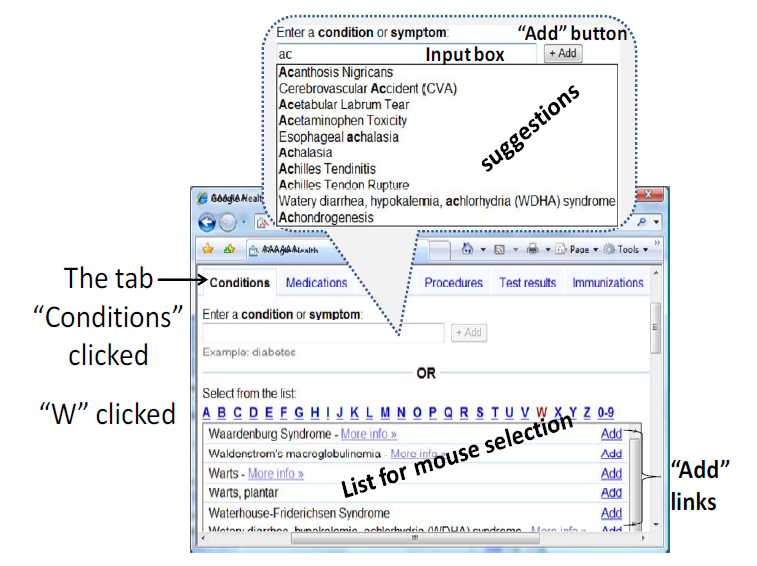
\includegraphics[width=0.7\textwidth]{fig/WebSideChannelExample1.png}
		\caption{Example Health Record System from \cite{WebSideChannel}}
		\label{Fig: HealthRecordSystem}
	\end{figure}
	
	In this example, the authors demonstrated that according to which tab or alphabet the user has clicked, the server returns a series of  packets with distinguishable lengths and directions. Further more, distinguishable packet traces can also be observed when user types in the input box triggering auto suggestion. As a result, an eavesdropper can deduce the user input simply by looking at the packet features of encrypted traffic.
\end{example}

\begin{example}
	The second vulnerable website is an online taxing service. In this system, the tax application form varies due to the payee's family status. The vulnerability of this website is that users are directed to different pages according to the form they are going to fill, while different pages results into packets of different lengths and directions, allowing an eavesdropper to reveal the family status of the user. The packet features of encrypted traffic again breached the data confidentiality.
\end{example}

%Financial Graph Example

%Search Keyword Example (briefly, refers to the other one)

\subsection{Traffic Analysis Countermeasures}




\section{Methodologies in Information Leakage }


\chapter{Experiment Setup} \label{Chp: Experiment Setup}
%All experiments are done within the Cooja simulator. The environment we simulated is as described in \Cref{fig: Setup}.

In this chapter we describe how we set up our experiments. The related source code can be downloaded from: \url{https://github.com/Salties/MyRepository} .

\section{Overview}

\Cref{Fig: Experiment Setup} illustrates an overview of our experiment setup. 

\begin{figure*}[h!]
	\center
	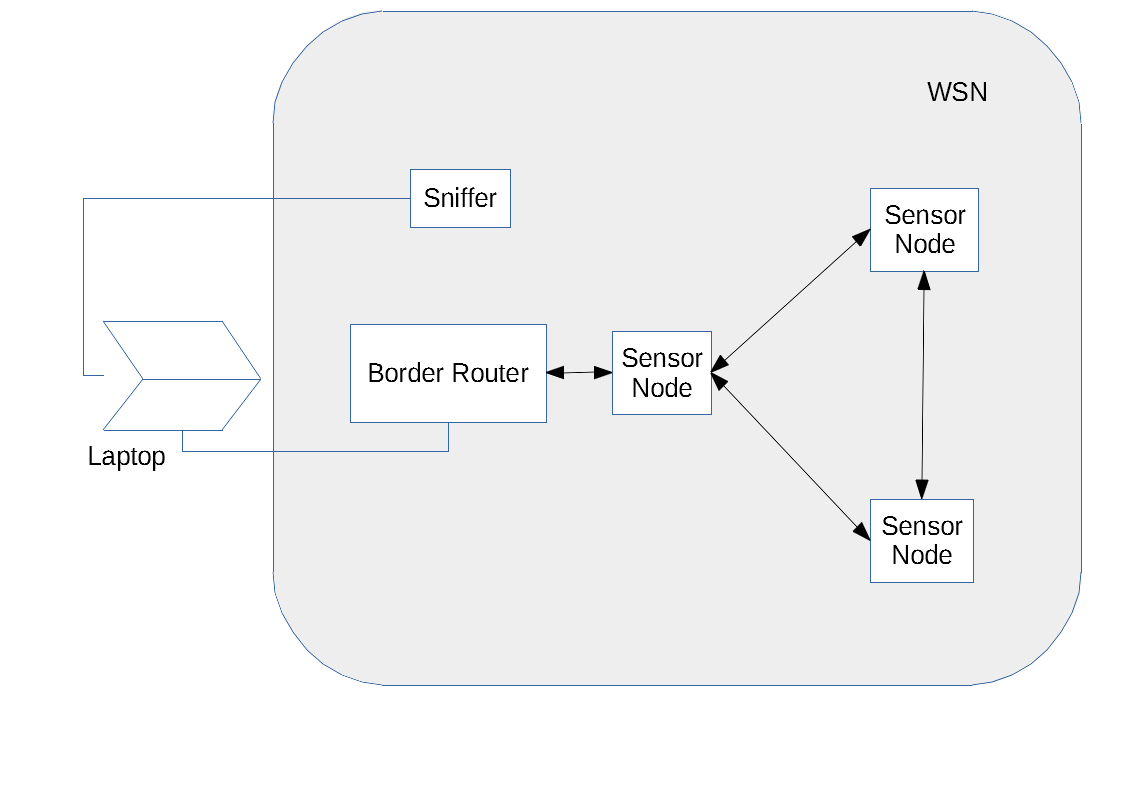
\includegraphics[width=0.75\textwidth,]{fig/setup.png}
	\caption{Experiment Setup} \label{Fig: Experiment Setup}
\end{figure*}

\begin{description}[style=nextline]
	\item[WSN]
	The greyed area on the right inside the rectangle of \Cref{Fig: Experiment Setup} represents a 6LoWPAN network as described in \Cref{Chp: Building Blocks}. The topology is dynamic as explained in \Cref{Sec: Network Layer}.  We make no further assumptions about the application for generality in this report.
	
	\item[Sensor Node]
	Each Sensor Node is a WSN device that supports the protocol suite described in \Cref{Tbl: Summary of WSN Building Blocks}. All Sensor Nodes are connected to the same 6LoWPAN network. We do not impose the use of CoAP in our setup; instead, we consider applications may directly invoke UDP (or DTLS) interfaces. 
	
	\item[Border Router]
	Border Router is a special instance of Sensor Node. Comparing to normal Sensor Nodes, Border Routers are specifically used to bridge other devices to the Sensor Network. In our experiments, Border Routers are connected to Laptops through USB connections. From a perspective of other Sensor Nodes in the WSN, a Border Router appears no different to the others. In many real world applications, the Border Router is connected to a management machine and serves as the DODAG root, but this is not necessarily the case in our experiments.
	
	\item[Sniffer]
	Sniffer is another special instance of Sensor Node. The Sniffer passively captures all frames it receives and does not transmit anything at all; thus it is transparent to other Sensor Nodes in the network. In our setup as of \Cref{Fig: Experiment Setup}, the Sniffer pipes any frames it captured to the Laptop. From a practical aspect, the hardware device of a Sniffer has a limited effective radius and thus would not be able to capture all frames in wide range WSNs; however this can be easily overcame by deploying multiple Sniffers to cover a wider area. In our experiments, we simply assume every frame in the WSN is visible to the Sniffer.
	
	\item[Laptop]
	The Laptops in our experiments usually represent adversaries with unequally supreme resources comparing to the Sensor Nodes in terms of energy, memory and computational power. In our setup of \Cref{Fig: Experiment Setup}, the Laptop, which represents an adversary, has access to all traffic captured by the Sniffer and is allowed to interact with other Sensor Nodes if the Border Router is compromised through external methods.
\end{description}

\section{Operating System}

We use Contiki\cite{Contiki} to build our experiments.  Our source codes are tested with Contiki release-3.0 which is available at: \url{https://github.com/contiki-os/contiki/releases/tag/3.0} .

\subsection{Brief Introduction to Contiki:}

The official instruction for using Contiki is available at:	\url{http://www.contiki-os.org/start.html} .


Contiki is an open source embedded system crafted for IoT devices. It has a good support on many recent hardware and it is optimised for code size. Contiki does not provide any direct User Interfaces, UI, by default. Instead, the embedded system provides a framework for developers to use C language to write (mostly) hardware portable codes, as well as providing a set of APIs including clock library, simple process management and network interfaces, etc.

To use Contiki, there are basically three steps:

\begin{enumerate}
	\item Write the application code in C. There are plenty examples in Contiki source code those can be used as frameworks.
	\item Compile the source code according to the target device through \textit{make} command. Note that the root of Contiki source code must be correctly specified in the \textit{makefile}. 
	\item Upload (also called ``burn'') the binary code to your device. 
\end{enumerate}

The application code is automatically executed whenever the device is powered on.

\section{Devices}

Three platforms are adopted in our experiments:

\begin{itemize}
	\item \textbf{TelosB}\cite{TelosB}, also known as Sky mote. This is a popular device for WSNs featuring low cost. As a trade off, TelosB has only very constrained performance in terms of bandwidth, available code size and processing power.
	
	\item \textbf{CC2538}\cite{CC2538}. This is a relatively powerful platform with an ARM-Cortex M3 processor. To our knowledge, this is one of the becoming dominant device used in WSN applications.
	
	\item \textbf{Wismote}\cite{Wismote}. This platform can be considered as a performance upgraded version of TelosB. Note that we only use Wismote in simulator. When using our code, one needs to modify the Contiki compiling system follow the instructions in: \url{https://github.com/contiki-os/contiki/wiki/MSP430X} .
\end{itemize}

All these nodes are 802.15.4\cite{802154} compatible and does not have any sensor attached by default. We omit further hardware details as it is beyond the scope of this project. 

\subsection{Cooja Simulator}

The Contiki source code includes the Cooja simulator under its tools folder. The official instruction for using the Cooja simulator is available at: \url{http://www.contiki-os.org/start.html} .

Cooja provides simulation for a whole WSN application. It generates simulated data for serial output, LED status and radio traffic, etc. An example of Cooja simulation is shown in \Cref{Fig: An Example of Cooja Execution}.

\begin{figure*}[h!]
	\center
	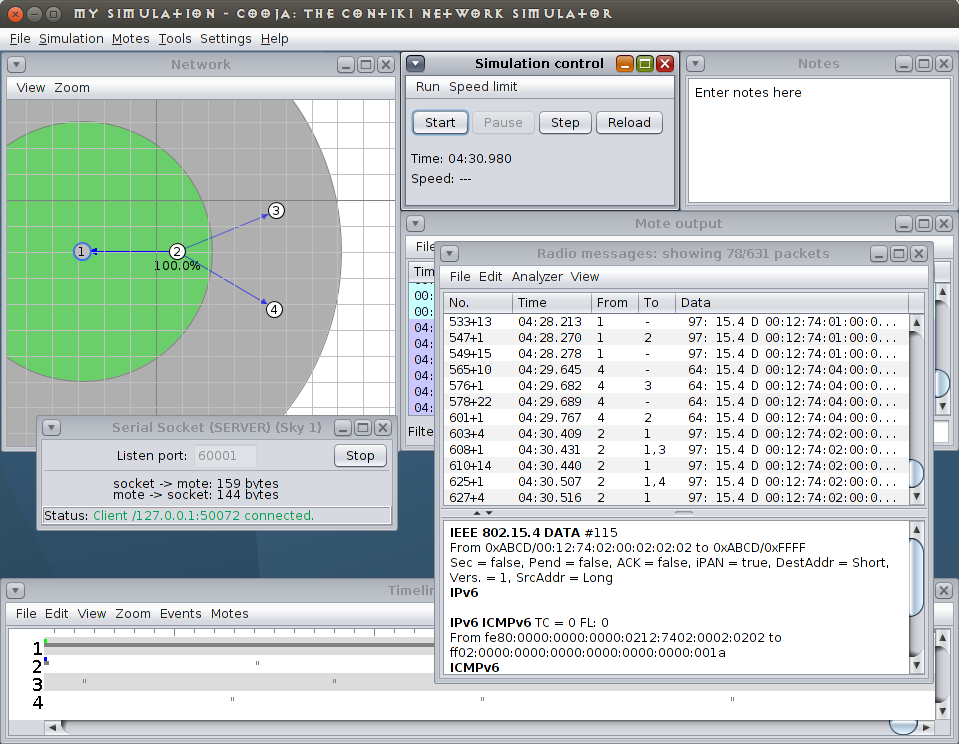
\includegraphics[width=0.8\textwidth]{fig/cooja_example.png}
	\caption{An Example of Cooja Execution}
	\label{Fig: An Example of Cooja Execution}
\end{figure*}

\Cref{Fig: An Example of Cooja Execution} shows a simulation simulating the exact same WSN topology as described in \Cref{Fig: Experiment Setup}, with \textcircled{1} being the Border Router. 

In this project, we are mostly interested in the radio traffic. The traffic is captured by the ``Radio messages'' plugin which exactly serves as the Sniffer in \Cref{Fig: Experiment Setup}. The corresponding pcap file is written by Cooja alongside the simulation under ``cooja/build/'' folder, which can later be opened by Wireshark\cite{Wireshark} for analysis, as shown in \Cref{Fig: A Wireshark Example}.

\begin{figure*}[h!]
	\center
	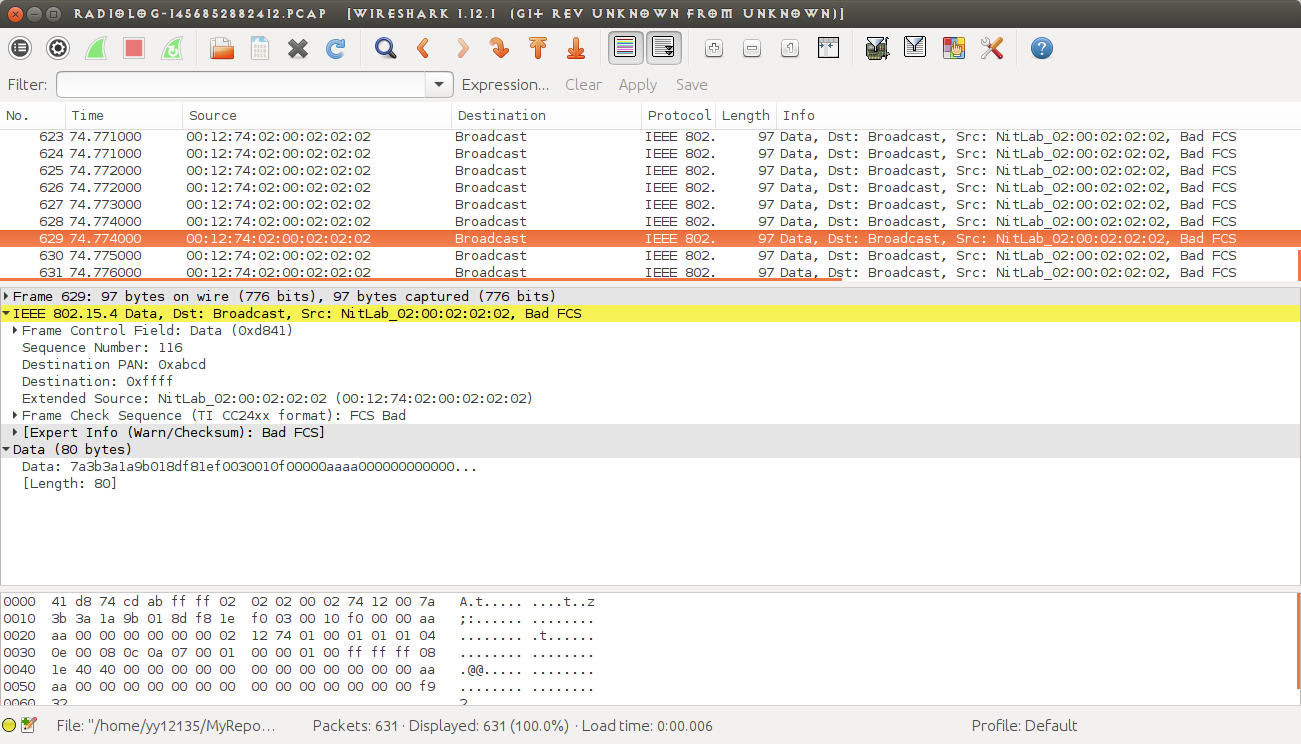
\includegraphics[width=0.8\textwidth]{fig/wireshark_example.png}
	\caption{A Wireshark Example}
	\label{Fig: A Wireshark Example}
\end{figure*}

As of the time of writing this report, Cooja in Contiki release-3.0 supports simulations for TelosB and Wismote. CC2538 is not yet supported in the latest version.

Cooja is not suitable for large scale experiments as there is a potential memory leakage problem which drastically downgrades long time simulations, or sometimes even crashes them. Also notice that the performance of Cooja is obviously better on low performance devices. For example, simulations with TelosB are nearly 8 times efficient than Wismote for the same application code.

\section{Security Measures}

In this report, we analyse traffic that is protected by two security measures implemented on Contiki release-3.0, namely noncoresec and DTLS.

\subsection{noncoresec}

In Contiki source code, LLSEC is an alias for \textit{noncoresec}.

\textit{noncoresec}\cite{noncoresec}\cite{LLSEC} is a reduced 802.15.4 Security implementation on Contiki. \textit{noncoresec} uses a hard coded network shared key that is defined by the ``NONCORESEC\_CONF\_KEY'' macro in ``project-conf.h'' file; thus it cannot be updated during runtime. 

When \textit{noncoresec} is enabled, we always assume it uses the highest Security Level (7), i.e. all frames are encrypted and authenticated in AES-128-CCM* mode with 16 bytes MAC, as described in \Cref{Subsec: 802154 Sec}. With this Security Level, all Sensor Nodes in the WSN must have the same key that is hard coded during compilation. External Sensor Nodes without the key cannot send or receive any frame and thus are repelled from the network.

In scenarios where the WSN is protected by \textit{noncoresec}, we always assume the adversary has no knowledge of the key. This effectively indicates that the adversary is unable to join the network at all since he cannot receive or send any frames as we explained above.

Our code using \textit{noncoresec} are successfully tested on all our devices. However, even though CC2538 has an AES coprocessor built in, the current version of Contiki code does not utilise this feature at all; instead, it uses a textbook software AES implementation as on other platforms. Also notice that the source code of \textit{noncoresec} is only included for TelosB platform by default. When using on other platforms, the developer needs to manually add its source code into the platform specific building system.

\subsection{DTLS} \label{Subsec: Experiment DTLS}

DTLS in Contiki is supported by a third party module \textit{tinydtls}\cite{tinydtls}. \textit{tinydtls} is originally developed for desktop systems and is later ported to Contiki. In the current version tinydtls-0.8.2, there are two cipher suites supported:

\begin{enumerate}
	\item TLS\_ECDHE\_ECDSA\_WITH\_AES\_128\_CCM\_8\cite{rfc7251}
	\item TLS\_PSK\_WITH\_AES\_128\_CCM\_8\cite{rfc6655}
\end{enumerate}

The use of cipher suite can be configured at compiling time by using the ``configure'' script under ``tinydtls-0.8.2'' folder. Also notice that when used with Contiki, ``--with-contiki'' argument is also required when running this script. By default, TLS\_ECDHE\_ECDSA\_WITH\_AES\_128\_CCM\_8 is preferred by the tinydtls implementation.

The keys (or master secrets) can be configured at runtime by using an interface provided by the tinydtls module. When using TLS\_PSK\_WITH\_AES\_128\_CCM\_8, where PSK stands for Pre Shared Key, the same master secrets must be coded beforehand into the clients and servers, or derived by external key management schemes.

The code from the tinydtls official website cannot be directly used on our platforms. The ``tinydtls-0.8.2'' folder in our source code contains a version of code we have tuned for our platforms. When using our code, the following problems should be noticed:

\begin{enumerate}
	\item TelosB does not support tinydtls as the code is oversized and cannot fit into the ROM of this device. Also notice that it cannot transmit frames longer than 127 bytes neither; thus any DTLS handshake message need avoid this type of Sensor Nodes in its path, as packets exceeding this length will be silently dropped by these nodes.
	\item Wismote with TLS\_ECDHE\_ECDSA\_WITH\_AES\_128\_CCM\_8 causes a crash of simulator. We have not yet figure out the exact cause of this problem. A potential cause might be illegal memory access in arithmetic operations.
	\item MTU specified by 802.15.4 Standard is 127 bytes whilst several DTLS handshake messages exceed this limitation. This constriction can be loosen by specifying\\ UIP\_CONF\_BUFFER\_SIZE, QUEUEBUF\_CONF\_NUM and UIP\_CONF\_RECEIVE\_WINDOW macros in ``project-conf.h'' file to a larger value. Nevertheless, specifying larger MTU does not guarantee the success transmission of packets. The handshake packets exceeding 127 bytes would still potentially be silently dropped during runtime.
	\item The handshake packets retransmission should be avoided at best effort. The restransmission implementation of tinydtls should not be relied on as sometimes it is not triggered by a packet lost, potentially due to a signal loss in the Contiki kernel. When a packet is lost during the handshake, the client and server will potentially freeze, resulting into a deadlock. Our current solution is to simply restart the procedure from the beginning, or simply reboot the devices.
	\item TLS\_ECDHE\_ECDSA\_WITH\_AES\_128\_CCM\_8 has a performance issue. Even on CC2538, each curve computation costs roughly 80 seconds on each side. This performance issue somehow triggers other problems in a chain reaction resulting into malfunctioning of the application code. The first problem is that the computation time exceeds the DTLS timeout, which therefore triggers the retransmission problem we described above. We have solved this problem in our code by increasing the timeout. The second problem happens when using  unequal computational power on client and server side, e.g. trying to perform a DTLS handshake from the Laptop through Border Router as the client to a CC2538 Sensor Node in the network. The unequal computational power leads to the fact that the Laptop processes the handshake packets immediately and continuously sends out the responses, without waiting for the Sensor Node to complete its computation. Consequently, the buffer of Sensor Node is instantly over flooded by the handshake packets resulting into some of them being dropped, which, again, triggers the problems caused by retransmission we described above. Our solution to this problem is to simply add a \textit{getchar()} into DTLS client of the Laptop side, of which asks a key stroke before sending each packet
%	\item Multi sessions is not well supported in the current tinydtls implementation on Contiki due to some memory management problem. In another word, try not to establish multiple DTLS sessions with one DTLS server running on the same Sensor Node. Further more, there is a potential memory leakage in tinydtls on termination of a DTLS session, which therefore could potentially crash the application or simulation. 
\item tinydtls is designed with asynchronous I/O. One must carefully designs the application code to use it.
\end{enumerate}

In experiments with DTLS, we consider the adversary is a group of compromised Sensor Nodes in the WSN. In other words, not only having all access to packet transmitted over the network, the adversary is capable to send any crafted packets to any Sensor Node in the network as well. In experiments with TLS\_PSK\_WITH\_AES\_128\_CCM\_8 being the cipher suite, we assume the adversary has no knowledge of the pre shared keys in any other paired Sensor Nodes; otherwise any ciphertext is immediately broken. Similarly, when TLS\_ECDHE\_ECDSA\_WITH\_AES\_128\_CCM\_8 is used, we assume the adversary has no knowledge of the private keys in other Sensor Nodes. In reality, such compromised Sensor Nodes can be Border Routers connected to adversary controlled Laptops deployed among the WSN. .

\subsection{Overloading noncoresec and DTLS}

Theoretically, it is possible to overload noncoresec with DTLS since they are implemented at different layers in the protocol stack. In another word, one can technically use noncoresec to provide MAC Layer security while using DTLS to provide Application Layer security.

However, in Contiki we noticed that either of them de facto adopts AES-128 with CCM mode as the underlining encryption method. Cryptographically speaking, the encryption part of AES-128 with CCM can be viewed as a pseudo random bit stream generator and overloading both of them is equivalent to use another pseudo random bit stream that is the XOR of them. To our knowledge, it is unclear whether this provides more randomness or not. However, intuitively under the assumption that AES-128 can be viewed as a pseudo random function, we argue that this overload does not seem to provide any more confidentiality. The same applies to the CBC-MAC.

On the other hand, the performance impact of overloading cannot be ignored in WSNs. In fact noncoresec and DTLS adds 23 bytes and 21 bytes overhead to each packet respectively whereas the MTU specified by 802.15.4 Standard is only 127 bytes, overloading them will immediately adds great overhead in terms of bandwidth and thus energy consumption. 

Hence, we argue that overloading is not practical and thus is excluded from our experiments.

\section{Applications} \label{Sec: Applications}

In this section we explain some simple applications we have developed in our experiments. These applications are aimed to cover the most generic scenarios of WSN applications. The source code of the applications are located in the ``experiments'' folder in our source code. 

\begin{description}[style=nextline]

	\item[{dtls-telnet}]
	This tool is a DTLS client runs on Linux. It establishes a DTLS session with a DTLS server and runs a telnet application that reads and sends data in ASCII. We use this tool in most of our experiment as the DTLS client. It is located under the ``tools'' folder in our source code.
	
	\item[{dtlsbr}]
	{dtlsbr} is a DTLS echo server merged with a Border Router application running concurrently. An echo server echoes everything received from the clients similar to PING. {dtlsbr} is developed to study how the tinydtls implementation affects the packet features.
	
	\item[{borderest}]
	{boderest} is a CoAP server merged with a Border Router application running concurrently. This application is used to predict some traffic features with CoAPs. Even though there is no security measure adopted in this application, we expect that most of the packet features should be linearly preserved with CoAPs as we explained in \Cref{Subsec: CoAPs}. This application is not compatible with TelosB due to code oversize.
	
	\item[{keydtls}]
	{keydtls} is developed to study how different DTLS session keys affect the packet features. The Sensor Node runs a DTLS server and reads client input, responses with a random string in ASCII representing a sensor reading.
	
	\item[{keyllsec}]
	{keyllsec} is developed to study how different noncoresec keys affect the packet features. There are two sub-applications in this application:
	\begin{itemize}
		\item \textbf{broadcast} application broadcasts an arbitrary message periodically.
		\item \textbf{unicast-sender} and \textbf{unicast-receiver} are a pair of applications where the sender periodically pushes an arbitrary message to the receiver.
	\end{itemize}
	These applications are protected by noncoresec.

	\item[{dtlseiri}]
	\textit{dtlseiri} is developed to study how the execution time of code on a DTLS server affects the time interval of response. Similar to {keydtls}, {dtlseiri} repeatedly calls the Contiki random number generator to generate a random ASCII string as response, representing a sensor reading with additional processing. The execution time is controlled by the number of calls to the random number generator. 

%application detection dtls PINGLOAD
	\item[{dtlspingload}]
	This application is identical to \textit{dtlseiri} but developed for a different purpose. It is used to study a potential side channel attack we named ``pingload'' which we explain in later chapters.
\end{description}

\section{Summary}

In this chapter, we described how our experiments are set up. Two security measures are used in our experiments, namely noncoresec and DTLS. 

We summarise the compatibility of the security measures to the platforms in our experiments as \Cref{Fig: Compatibility of Platforms and Security Measures}.

\begin{table}[h!]
	\center
	\begin{tabular}{|c|c|c|c|}
	\hline
	\multirow{2}{*}{} & \multirow{2}{*}{noncoresec} & \multicolumn{2}{c|}{DTLS} \\ \cline{3-4} 
	                  &                             & ECDHE\_ECDSA & PSK        \\ \hline
	TelosB            & \checkmark                  & N/A          & N/A        \\ \hline
	CC2538            & \checkmark                  & \checkmark   & \checkmark \\ \hline
	Wismote           & \checkmark                  & N/A          & \checkmark \\ \hline
	\end{tabular}
	\caption{Compatibility of Platforms and Security Measures}
	\label{Fig: Compatibility of Platforms and Security Measures}
\end{table}

We have also developed several simple applications to model the most typical WSN application scenarios. We summarize their compatibility in \Cref{Fig: Compatibility of Platforms and Applications}.

\begin{table}[h!]
	\center
	\begin{tabular}{|c|c|c|c|c|c|c|}
	\hline
	\multirow{2}{*}{} & noncoresec & \multicolumn{4}{c|}{DTLS}                           & No Security \\ \cline{2-7} 
	                  & keyllsec   & dtlsbr     & keydtls    & dtlseiri   & dtlspingload & boderest    \\ \hline
	TelosB            & \checkmark & N/A        & N/A        & N/A        & N/A          & N/A         \\ \hline
	CC2538            & \checkmark & \checkmark & \checkmark & \checkmark & \checkmark   & \checkmark  \\ \hline
	Wismote           & \checkmark & \checkmark (*) & \checkmark (*) & \checkmark (*) & \checkmark (*)   & \checkmark  \\ \hline
	\end{tabular}
	\caption{Compatibility of Platforms and Applications}
	\label{Fig: Compatibility of Platforms and Applications}
	(*): As explained in \Cref{Subsec: Experiment DTLS}, on Wismote DTLS can only be used with\\ TLS\_PSK\_AES\_128\_WITH\_CCM\_8.
\end{table}



%A table for available combinations

%\begin{itemize}
%\item{\bf Adversary} is a malicious party that tries to illegally reveal information from the encrypted traffic.
%\item{\bf Border Router}, or BR, is a device that connects adversary to the sensor network. \textbf{BR is not allowed when LLSEC is enabled} as the adversary does not have the key and hence cannot connect into the network. We will discuss more about LLSEC in \Cref{Chp: LLSEC}.
%\item{\bf Sniffer} passively captures all traffic in the network. 
%\item{\bf Target} and {\bf Nodes} are sensors deployed in the sensor network. They communicates to each other through encrypted channels.
%\item{\bf Sensor Network} discussed in this paper is a 6LowPAN network based on Contiki OS.
%\end{itemize}

%Realistically speaking, this scenario could happen say an adversary sitting near a smart house with a laptop attached to a SoC\footnote{System on Chip} device, or your malicious neighbour walks into your smart house with her smart phone.
%
%\section{Adversary Power}
%The powers assumed in the experiments are considered to be practical in real life.
%
%When LLSEC is enabled, all traffic, including RPL\footnote{Routing Procol for Low-power and Lossy Networks} messages, are encrypted; therefore no external nodes can connect to the network as an external node cannot send any valid RPL messages to join the network. The adversary only passively sniffs all traffic.
%
%With LLSEC disabled, the adversary can therefore join the sensor network through a BR and hence is also capable to send messages to the target(s). However, she will not be able to inject any message into an encrypted channel such as a DTLS channel.
%
%\section{Types of Packets}
%We simply categorise the packets into two types:
%\begin{itemize}
%\item {\bf Network Management Packets}: These are the packets generated by the protocols to  maintain the functionality of network, such as MAC ACKs, RPL messages or ICMP messages.
%\item {\bf Data Packets}: These are those packets generated by applications running on sensor nodes., such as a CoAP packet.
%\end{itemize}
%
%This is only a subjective rough categorisation and may not be precise. For example an TCP data packet may set its ACK flag, or DTLS handshake packets could ambiguously fall into both categories. However, we ignore this ambiguity as it is not our focus.
\chapter{Potential Leakage Sources}

In this chapter, we discuss the potential leakage sources in the experimental environment we have set up in \Cref{Chp: Experiment Setup}. 

\section{A Review of Review}
%What is ``Information''

The first and fundamental question that must be clarified in this project is: what is ``information''?

If we look at those attacks described in \Cref{Chp: Literature Review}:

\begin{itemize}
	\item In literatures about the flaws in implementations of algorithms and protocols, ``information'' is the plaintext, usually represented as a numerical value, such as \cite{802154sec} \cite{rfc7457} \cite{CompressionRatioAttack} \cite{PaddingOracle}. Or it could be the secret key materials in many cryptographic side channel attack literatures, such as \cite{DPA}.
	\item In Traffic Analysis Attacks against web applications, ``informaiton'' is the user input, such as \cite{PinpointWeb} \cite{SearchAttack}, or the content of websites such as \cite{WebSideChannel}.
	\item When we talk about website fingerprinting such as \cite{WebsiteFingerprint} \cite{Peekaboo} and \cite{PClassifier}, ``information'' is the identity of websites. 
	\item The category only gets even more messy and trivial when we look at other Traffic Analysis Attacks, such as the spoken language and phrases in \cite{VoIPLanguage} and \cite{VoIPPhrases}, user event and OS of Apple product in \cite{AppleMessage} or even the ambient change and motion event in \cite{Video}.
\end{itemize}

``Information'' is always a relative concept to ``application'', so is ``leakage''. 

In this report, we are interested on information leakages with regard to the following attributes:

\begin{description}[style=nextline]
	\item[Content and Size of Application Data]
	The implication of Application Data varies on different applications.
	
	\item[Cryptographic Key]
	This represents the corresponding key materials in the security measure.
	
	\item[Application Code Routine]
	This implies the application specific feature.
	
	\item[Network Topology]
	This implies how Sensor Nodes connect to each other.
\end{description}

Notice that the information leakage is highly application specific. In this report, we discuss only the applications described in \Cref{Sec: Applications}. 

\section{Observables}

Generally speaking, observables in captured traffic can be classified into two categories:
\begin{enumerate}
	\item Implicit observables. These imply the data an adversary can access without inspecting the content of packets.
	\item Explicit observables. These imply the data given in the unencrypted part of packets.
\end{enumerate}

\subsection{Implicit Observables}

There are mainly two observables we concern in this category:

\begin{description}[style=nextline]
	\item[Packet Size] 
	This refers to the size (or length) of a packet. This value is also explicitly included in the packet headers.
	
	\item[Packet Timing]
	This refers to the time being sent of a packet. 
\end{description}

In addition to Packet Size and Packet Timing, there are some other implicit observables we do not concern in this report:

\begin{description}[style=nextline]
	\item[Presence of Packets]
	Apparently, the presence of a packet implies the existence of a Sensor Node device, which is kind of an information leakage. However, we do not take this into account. We assume the adversary has prior knowledge of the existence of WSN.
	
	\item[RSSI]
	Receive Signal Strength Indicator, RSSI, indicates the RF signal strength from a Sensor Node. Practically speaking, by measuring the RSSI of frames sent from a specific source MAC address, the adversary is capable to reveal the physical location of Sensor Node. In this report we do not take RSSI into account as its physical character is beyond the scope of this project. We assume the adversary has prior knowledge of the geographic information of the Sensor Nodes.
\end{description}

\subsection{Explicit Observables}

We have explained in \Cref{Chp: Experiment Setup} that there are two security measures implemented on our platform, namely noncoresec and DTLS. Referring to \Cref{Chp: Building Blocks}, these measures are implemented at different layers. The observables are therefore different for noncoresec and DTLS. 

\subsubsection{noncoresec}

As explained in \Cref{Subsec: 802.15.4 Security Implementation in Contiki}, noncoresec is the 802.15.4 Security implementation on Contiki. When noncoresec is enabled, all captured frames is in the form we explained in \Cref{Subsec: 802.15.4 MAC} and \Cref{Subsec: 802154 Sec}. The MAC Layer Header is the only observable part of a packet.

We stated in \Cref{Subsec: noncoresec in experiment} that we always use highest Security Level of 802.15.4 Security; therefore:
\begin{itemize}
	\item MAC Payload is always authenticated and encrypted in AES-128 with CCM* mode.
	\item Security Level is constantly 0x7.
	\item Key Strategy is constantly 0x0 as noncoresec does not implement any key management.
\end{itemize}

As a result of MAC Payload being authenticated and encrypted, 
\begin{itemize}
	\item The adversary cannot join the 6LoWPAN network as we have explained in \Cref{Subsec: noncoresec in experiment}.
	\item The adversary cannot distinguish an IPv6 packet and an ICMPv6 packet by simply looking the contest as it is encrypted. The IPv6 packets effectively contained the Applicatoin Data. ICMPv6 packets in our set up is mainly RPL messages.
\end{itemize}

\subsubsection{DTLS}

When DTLS is used, 

\subsection{Traces}

\section{Theoretical Analysis}







\chapter{Link Layer Security}

\section{Non core security}

\section{802.15.4 security}

\section{Reset Problem}

\section{Distinctive packet length for RPL packets}

\chapter{DTLS}
DTLS has potentially the best interoperability as it is an variation of the widely used TLS in Internet. However, its design might not fit into the nature of WSN for practical reasons.

\section{Implementation Issues}
tinydtls\cite{tinydtls} currently supports two ciphersuites, namely TLS\_PSK\_WITH\_AES\_128\_CCM\_8 and TLS\_ECDHE\_ECDSA\_WITH\_AES\_128\_CCM\_8. 

However, we encountered several difficulties when trying to set up a  network with DTLS.

\begin{description}
\item[Low Computational Power] \hfill \\
Curve computation requires relatively a large amount of computational power. Even using a relatively power platform (CC2538), it still takes minutes to complete a DTLS handshake with
TLS\_ECDHE\_ECDSA\_WITH\_AES\_128\_CCM\_8.

\item[Low Bandwidth] \hfill \\
The 6LowPAN standard specifies that the minimum MTU is 127 bytes whilst 67 (87 with LLSEC) bytes are occupied by protocol headers until UDP, which leaves 60 (40 with LLSEC) bytes available for UDP layer payload. This value can be easily exceeded even during the handshake, such like using a longer key. Some attempts have been made to solve this issue, e.g. CoDTLS\cite{CoDTLS}\footnote{This draft has been abandoned for some reason we do not know.}.

\item[Code Size] \hfill \\
The tinydtls fails to fit into some devices, e.g. skymote, as its size of code is too large.
\end{description}

Therefore although TLS\_PSK\_WITH\_AES\_128\_CCM\_8 is less flexible (and probably less secure) as it uses a pre-shared master secret than TLS\_ECDHE\_ECDSA\_WITH\_AES\_128\_CCM\_8, it is still considered to be a relatively practical security measure as it requires less resources.

\section{No multicast support}
Some application protocols, such as CoAP, utilises the multicast feature of 6LowPAN whilst TLS is a protocol designated for securing communications between two parties, so is DTLS.

\section{Overloading DTLS with LLSEC}
Adopting both security measures at the same time is possible as they are implemented at different layers. However, it is questionable whether this will bring more security, as both {\it noncoresec} and TLS\_PSK\_WITH\_AES\_128\_CCM\_8 are using 128 bit AES with CCM mode as their cryptographic primitive.

\chapter{PINGLOAD: PING side-channel for Payload } \label{Chp: PINGLOAD}

Support of PING is required by \cite{rfc1122} and is also enabled in Contiki OS by default. In this chapter, we describe a potential timing attack to finger print the code routine on target Sensor Node through ICMP ECHO (PING) packets.

\section{Scenario Setting}

In this attack, we consider a different scenario where the adversary is connected into the 6LoWPAN network and is able to send packets to a specific Sensor Node. As we have explained in \Cref{Subsec: ICMPv6}, ICMP ECHO is not authenticated; therefore it is always possible for the adversary to PING any target node in the network. An overview of such scenario is as depicted in \Cref{Fig: Scenario of PINGLOAD}.

\begin{figure*}[h!]
	\center
	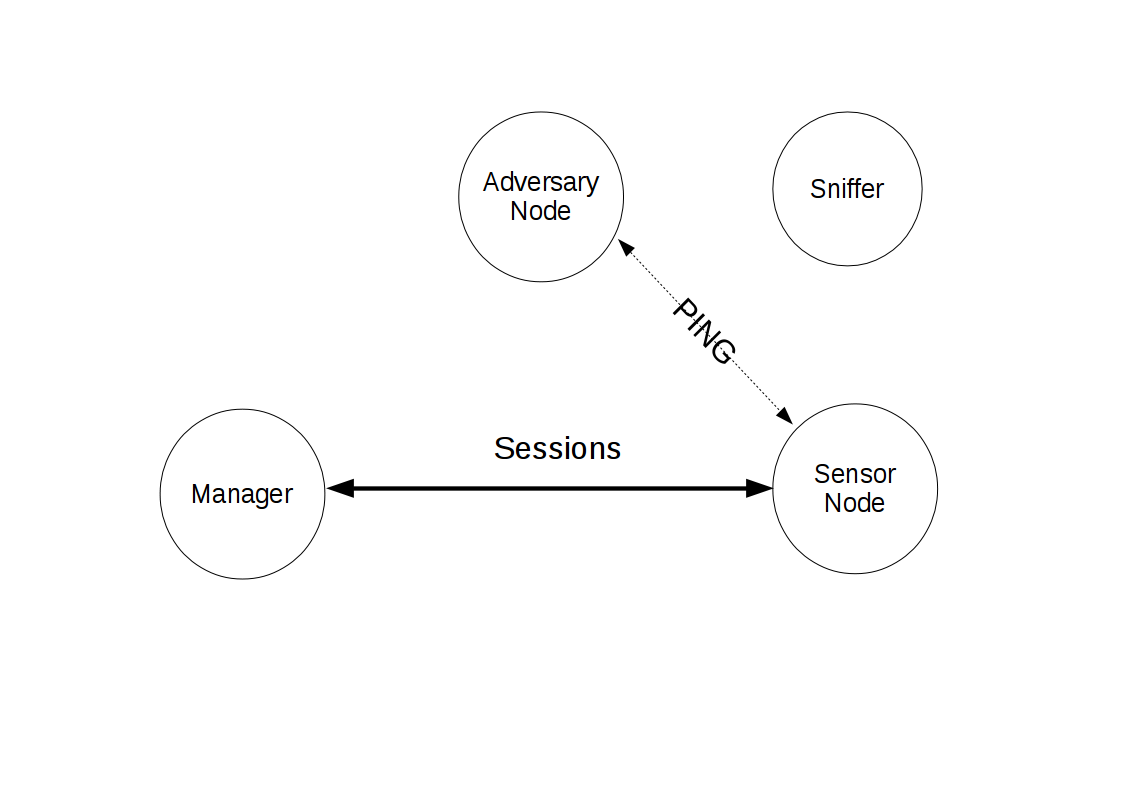
\includegraphics[width=0.8\textwidth]{fig/PINGLOAD_scenario.png}
	\caption{Scenario of PINGLOAD}
	\label{Fig: Scenario of PINGLOAD}
\end{figure*}

In this scenario, we assume the Manager engages with the target Sensor Node in Sessions. The Adversary Node is connected into the network and sends ICMP ECHO Requests (PING Request) to the Sensor Node. The Sensor Node, by default enabled by the Contiki system, replies with ICMP ECHO Responses (PING Respon. All packets are captured by the Adversary controlled Sniffer. \Cref{Fig: Time line of PINGLOAD} shows the time line of this scenario.

\begin{figure*}[h!]
	\center
	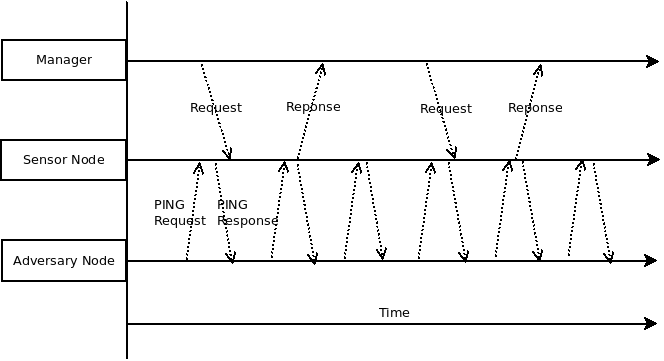
\includegraphics[width=0.8\textwidth]{fig/PINGLOAD_time.png}
	\caption{Time line of \Cref{Fig: Scenario of PINGLOAD}}
	\label{Fig: Time line of PINGLOAD}
\end{figure*}

\section{Phenomenon}

In our experiments, we realised that the latency between PING Request and PING Response varies according to the status of the Sensor Node. To be more specifically, the PING latency is apparently lower when the Sensor Node is not processing the Request sent by the Manager. The concept is shown in \Cref{Fig: Concept of PINGLOAD}. 

\begin{figure*}[h!]
	\center
	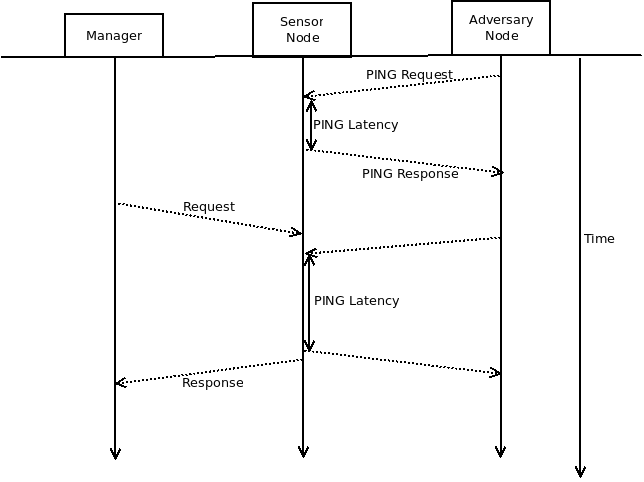
\includegraphics[width=0.9\textwidth]{fig/PINGLOAD_concept.png}
	\caption{Concept of PINGLOAD}
	\label{Fig: Concept of PINGLOAD}
\end{figure*}

This indicates that there is a potential leakage of the status of Sensor Node over the PING latency.

\section{Proof of Concept Experiment} \label{PoC PINGLOAD}

We set up a series of experiments to proof the potential of such side channel information leakage. The experiments are done in Cooja simulator with Wismote. The experiment WSN is set up as \Cref{Fig: Proof of concept experiment of PINGLOAD}.

\begin{figure*}
	\center
	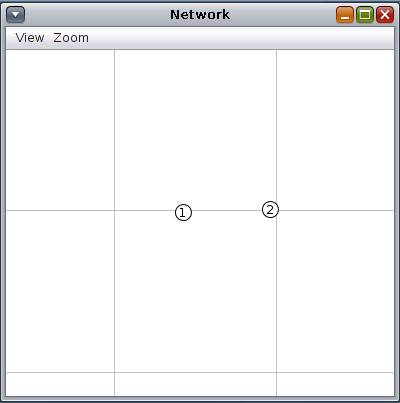
\includegraphics[width=0.5\textwidth]{fig/PINGLOAD_PoC.png}
	\caption{Proof of concept experiment of PINGLOAD. \textcircled{1} is a border router and \textcircled{2} is the target Sensor Node.}
	\label{Fig: Proof of concept experiment of PINGLOAD}
\end{figure*}

In this experiment, two procedure on our Linux host are used to simulate the Manager and the Adversary respectively. We argue this is equivalent to the settings of \Cref{Fig: Scenario of PINGLOAD} as we are evaluating the latency between PING Requests and PING Responses and thus the source of the PING Request is irrelevant in this experiment.

The target Sensor Node runs the dtlspingload application we explained in \Cref{Sec: Applications}. In this application, the Sensor Node establishes a DTLS connection with the Manager. Upon receiving a Request, the Sensor Node calls a ReadSensor() function to generate the data and replies that data to Manager, simulating a typical scenario in WSN. A overview of Session in this application is described as \Cref{Fig: A Session of dtlspingload}.

\begin{figure*}
	\center
	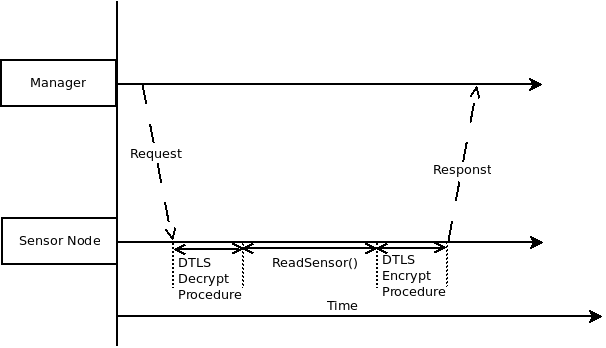
\includegraphics[width=0.8\textwidth]{fig/PINGLOAD_Session.png}
	\caption{A Session of dtlspingload}
	\label{Fig: A Session of dtlspingload}
\end{figure*}

Due to the unsynchronised clocks between the physical host and Cooja simulator, the Request from the Manager process and the PING Request from the Adversary process are sent to the simulated Wismote Sensor Node in random timings; therefore the event of the PING Request hitting the period of processing Request is unpredictable.Some of the packets are lost during the transmission.

For this experiment, we implemented three types of ReadSensor() functions.

\begin{description}[style=nextline]
	\item[Constant ReadSensor()]
	ReadSensor() returns a constant value as Response.
	\item[Random Number ReadSensor()]
	ReadSensor() calls the Contiki system random number generator for a number of times, and returns a random number as Response.
	\item[Arithmetic ReadSensor()]
	ReadSensor() does arithmetic operations on random numbers generated by the Contiki system random number generator, and returns the result as Response.
\end{description}

\section{Experiment Results}

Some tools are developed to analyse the result. The usage of the data and tools are described in \Cref{PINGLOAD Data}. The raw and pre-processed data are available at: 
\begin{center}
	\url{https://github.com/Salties/MyRepository/tree/master/experiments/dtlspingload/Data}
\end{center}

For simplicity, the term ``pingload'' refers to the collected PING latency data for a specific application as we described in \Cref{PoC PINGLOAD}.

\begin{definition}
	A trace of pingload is of the form:
	\begin{equation*}
		T=\{l_1, l_2, ..., l_n\}
	\end{equation*}
	where $l_i$ is the $i$-th PING latency in the experiment.
\end{definition}

We also use the term ``payload'' to denote the application code being executed on target Sensor Node.

\subsection{PING Latency Without Payload} \label{Sleep PINGLOAD}

As a base line comparison, we collected the pingload data from the helloworld application, i.e. the Sensor Node is put into eternal sleep after printing a line of ``Hello, world!''. In another word, there is no payload in this application.

Not surprisingly, the PING latencies are mostly small values between $12$ and $13$ ms. There is only one exception in the experiment which is $293$ ms. We suspect this is caused by the Sensor Node executing kernel code.

\begin{figure*}
	\centering
	\begin{subfigure}[b]{0.5\textwidth}
		\centering
		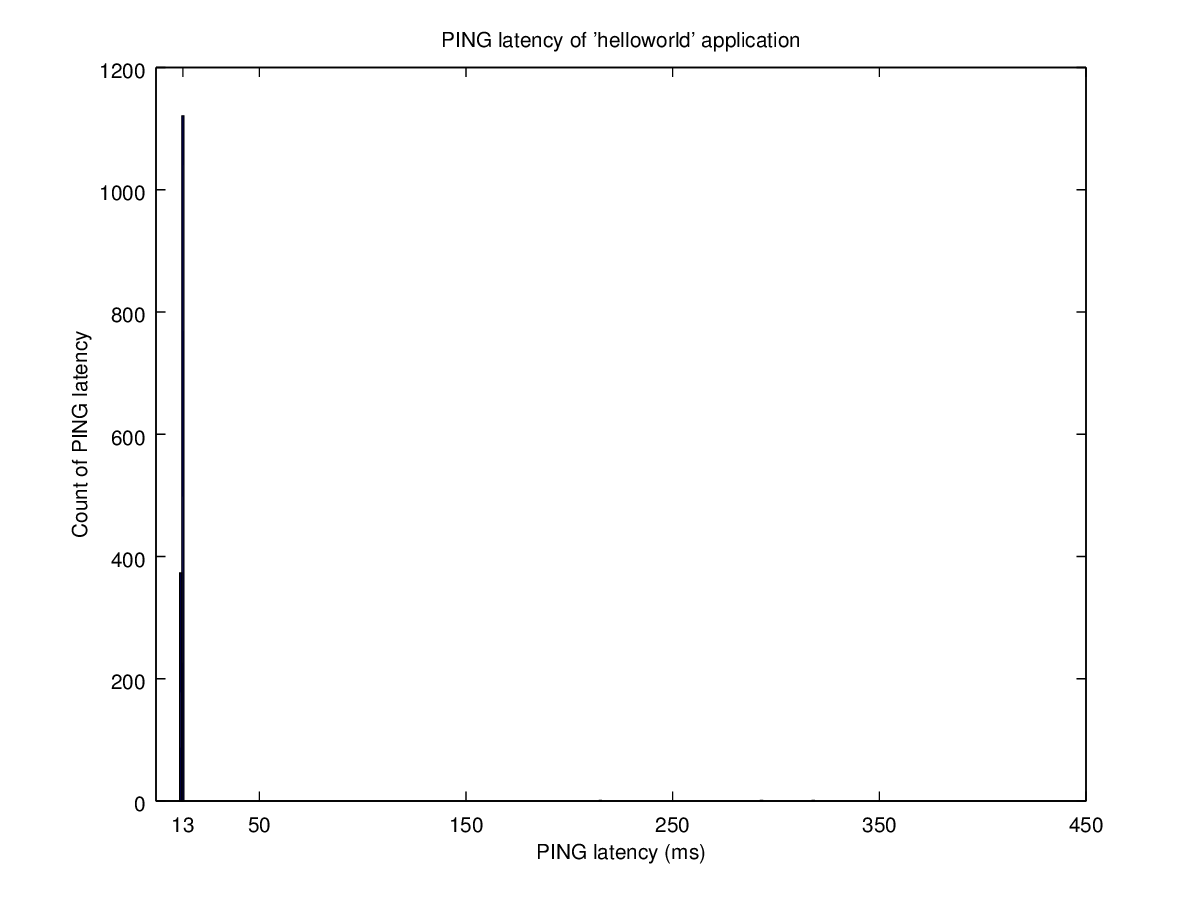
\includegraphics[width=0.4\textwidth]{fig/sleepRI.png}
		\caption{Histogram of helloworld pingload}
	\end{subfigure}
	\begin{subfigure}[b]{0.5\textwidth}
		\centering
		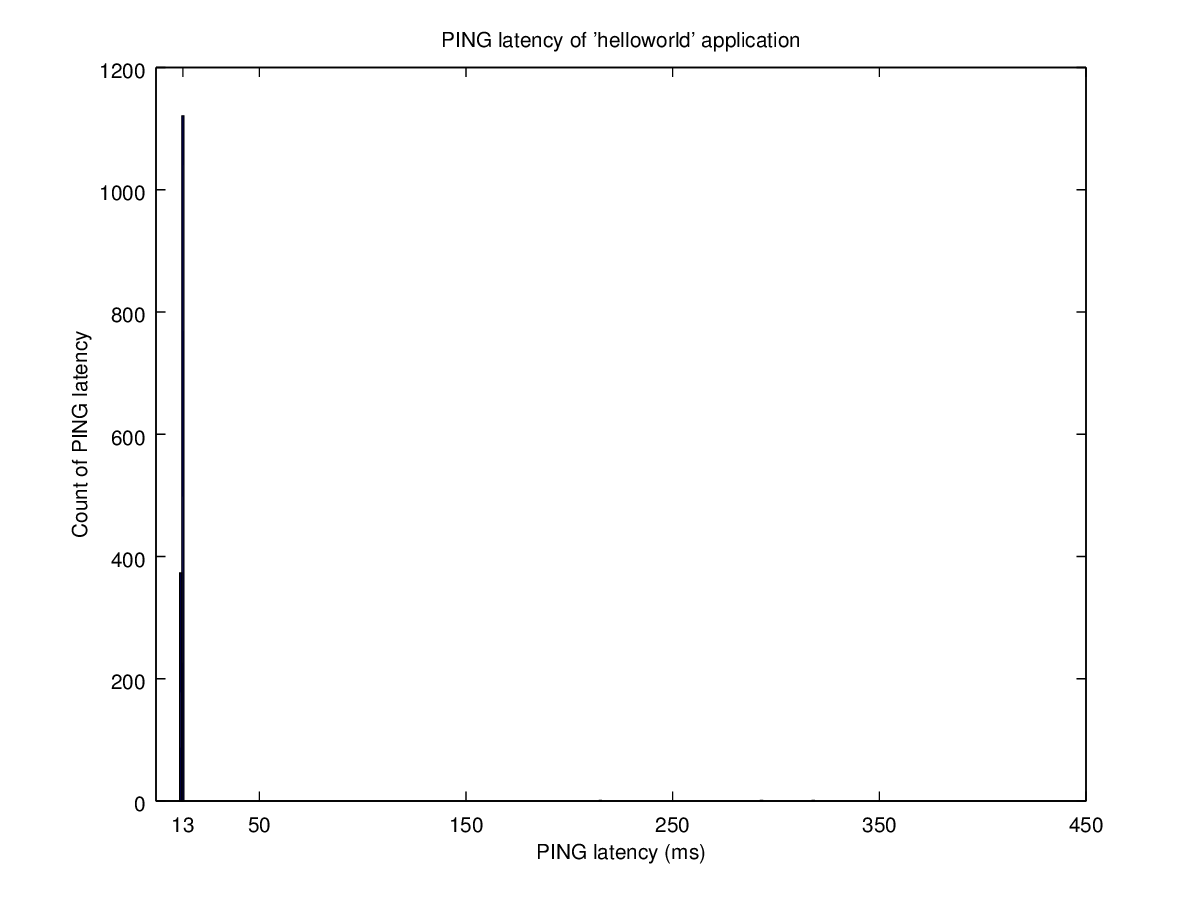
\includegraphics[width=0.4\textwidth]{fig/sleepRI.png}
		\caption{CDF of helloworld pingload}
	\end{subfigure}
\end{figure*}


%
%\subsection{Hypothesis} \label{Sec: pingload hypothesis}
%A phenomenon we realised is that when a PING packet arrived while the target node is executing some payload, say reading a sensor or processing data, the PING RIs begin to vary comparing to a stable value when no payload is given to the sensor node. 
%
%\begin{example}
%\begin{figure}
%\centering
%{
%  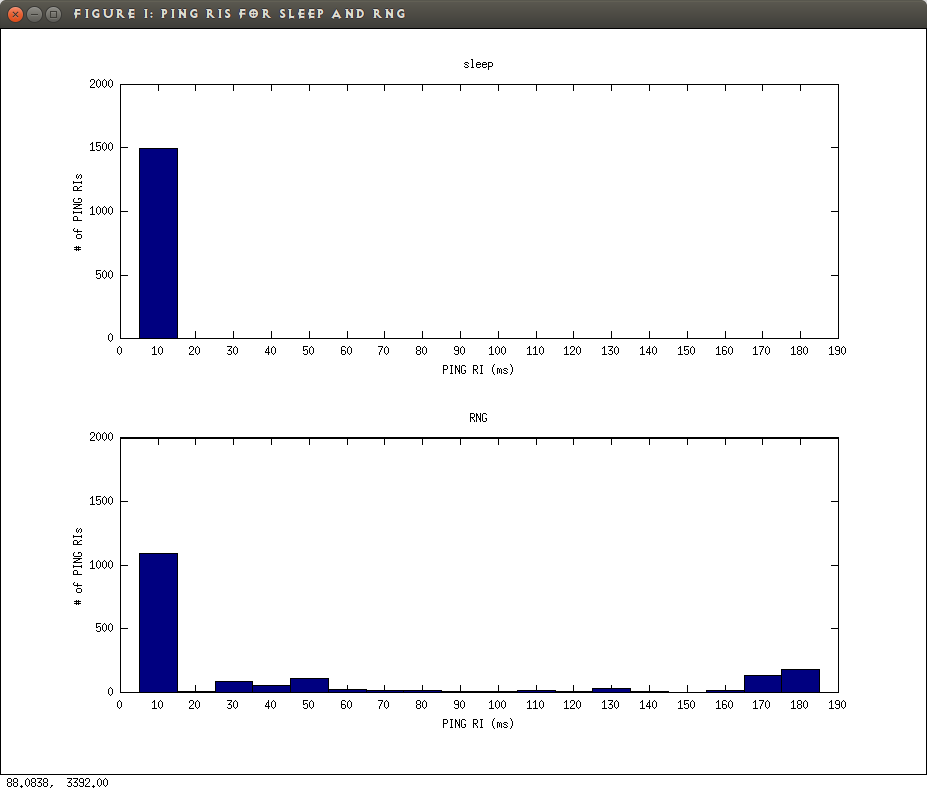
\includegraphics[width=1\textwidth]{fig/pingri.png}
%}
%\caption{An example of PING RIs with different payload}
%\label{Fig: PINGLOAD RIs}
%\end{figure}
%\Cref{Fig: PINGLOAD RIs} shows PING RIs collected in two experiments. In the upper half, the target node is constantly in asleep whilst in the lower half,  it occasionally receives a request which triggers the target to call RNG. We can see that the PING RI varies alongside the target is given some payload from this figure.
%\end{example}
%
%The data shown in \Cref{Fig: PINGLOAD RIs} suggests that the “plain”, that is without any interference, PING RI is 12 to 13 ms. Those variations of  shown in the lower half of \Cref{Fig: PINGLOAD RIs} is potentially caused by the payload on target.
%
%This result inspires us that the distributions of PING RIs might vary according to the payload on target and could possibly considered as a fingerprint to the target’s application. In other word, an adversary could possibly tell whether the target is running a specific application by looking at its PING RIs distribution.
%
%The attack then is strait forward:
%\begin{description}
%\item[Profile sleep RIs]: \hfill\\
%The PING RIs for a sleeping node of the same platform can be profiled by pinging a sleeping node. We denote the sleeping profile as $RI_{sleep}$. 
%
%\item[Fingerprint application]: \hfill\\
%The adversary collects PING RIs on a profiling node with known application. The profiling node needs to be of the same platform and executing the same code of the target’s. The profiled application fingerprint is a sample set of RIs, denotes as: $F_p=\{a_1, a_2, ... , a_n\}$ where $a_i$ is the RI of $i$th PING to the profiling node. 
%
%\item[Collect fingerprint of target]: \hfill\\
%The adversary then fingerprints the payload on the target in a similar way by pinging it. We denote the collected target sample set of RIs as: $F_t=\{b_1, b_2, ..., b_m\}$ where $b_j$ is the RI of $j$th PING to the target node.
%
%\item[Extract Featured RIs]: Since a node is usually in a sleep state, most of the PING RIs will hence results into $RI_{sleep}$. To improve the clarity of our fingerprint, we can remove them from the data sets and keep only the PING RIs those (seemingly) has been interfered by the payload. We denote the extracted RIs as \textbf{Featured RIs}:
%\begin{eqnarray*}
%F’_p = F_p - RI_{sleep} = \{x | x \in F_p,  x \notin RI_{sleep}\}\\
%F’_t = F_t - RI_{sleep} = \{x | x \in F_t,  x \notin RI_{sleep}\}
%\end{eqnarray*}
%
%Practically speaking, the PING protocol are designed to be responded immediately for diagnosis purpose; hence $RI_{sleep}$ usually has an extremely low variance and its mean is also much less than $F_p$ and $F_t$. Therefore we can ignore the error induced by wrongly removed packets.
%
%Using the Featured RIs not only provides a better vision of the fingerprint but also removes the error caused by different frequency of the target code being executed, as all the Featured RIs are  collected when the node is at a non-sleeping state. 
%
%\item[Estimate Distribution (Optional)]: \hfill\\
%We then estimate the distributions of $F’_p$ and $F’_t$, denote as $\mathbb{D}_p$ and $\mathbb{D}_t$. A naive method is to simply use their histograms. An example of such histograms are shown as \Cref{Fig: featuredri_rng}.
%
%\begin{figure}
%\center
%{
%	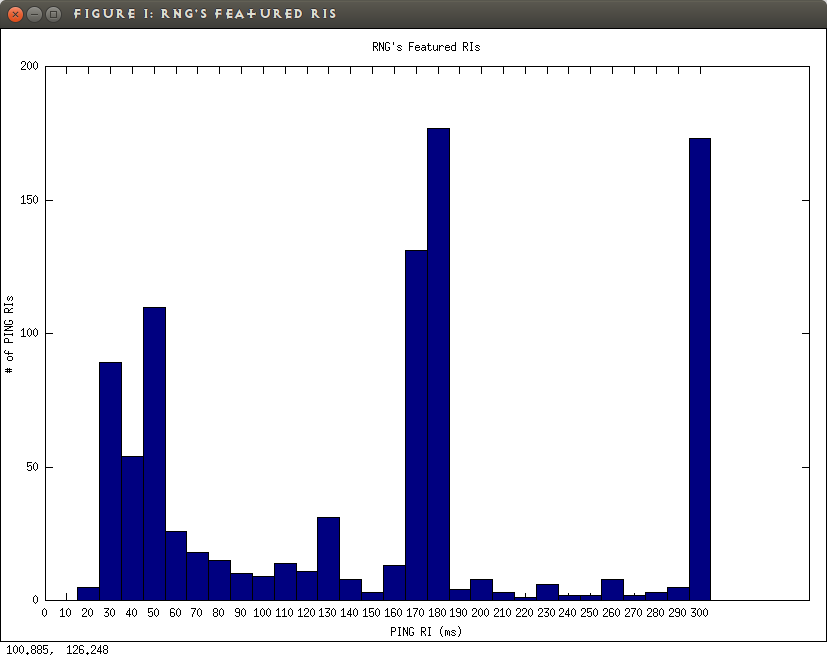
\includegraphics[width=0.49 \textwidth]{fig/featuredri_rng1.png}
%	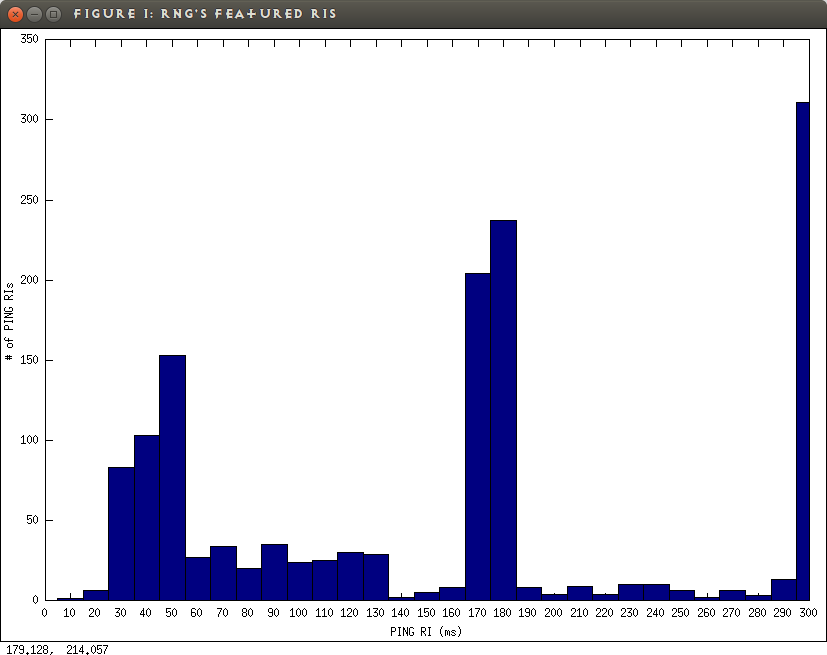
\includegraphics[width=0.49 \textwidth]{fig/featuredri_rng2.png}
%}
%\caption{Two examples of RNG’s Featured RIs histogram}
%\label{Fig: featuredri_rng}
%\end{figure}
%
%\item[Distinguish Distributions]: \hfill\\
%Finally we test whether $D_t$ and $D_p$ are the same distribution. A naive way is to compute the correlation of counts of the histograms. We conclude the target node is running the profiled application if $D_t$ and $D_p$ are the same distribution.
%\end{description}
%
%Practically speaking, the key point of Application Fingerprinting is to test whether the target’s Featured RIs is sampled from same distribution of the profiled one, i.e. whether $F’_t = F’_p$; therefore estimating their distribution might not be necessary for some statistical methods such as t-tests. However as we can see in \Cref{Fig: featuredri_rng}, PING RIs’ distribution are very unlikely to be normalised. Therefore a future work is to find a better distinguishing method than the current naive one.
%
%\subsection{Experiment Results}
%We tried our Application Fingerprinting attack in a Cooja simulated Wismote platform with different codes. \textbf{In conclusion, the fingerprint appears to be effective for certain circumstances but will tends to result into false positives as the profiled application and target application gets similar to each other.}
%
%To be more specifically, the target node execute some specific code upon receiving an application layer protocol request, similar to CoAP. Further more, all traffic are protected by DTLS with TLS\_PSK\_WITH\_AES\_128\_CCM\_8 ciphersuite. Both intervals of PINGs and the application request are set to some asynchronised value to avoid overflooding the target and to create a ‘more realistic’ simulation.
%
%Everything other than the examined code are the same for all experiments. Two samples are collected independently for each code to simulate a fingerprinting scenario. The histograms are clustered by 5ms from 0ms to 500ms.
%
%We examined two classes of codes:
%\begin{description}
%\item[RNG Calls]: \hfill\\
%The target node repeatedly calls RNG for $i$ times. We examined their Featured PING RI for different values of $i$. The reason for picking RNG is that on some platforms where a hardware RNG is provided, the call to it is expected to be similar to a call to a sensor reading which is actually an interrupt to the processor. Results are shown in \Cref{Tbl: pingload RNG}.
%
%\item[Arithmetic Operations]: \hfill\\
%The target node repeatedly does arithmetic operations, namely addition, multiplication and modular, on two randomly generated word size integers for 10000 times. This class is particularly interested from a cryptographic point of view as the number of arithmetic operations could potentially developed to key recovering attacks. Results are shown in \Cref{Tbl: pingload arth}.
%\end{description}
%
%
%
%\begin{table}
%\centering
%\begin{tabular}{|c|cccc}
%\hline
%\textit{\textbf{Correlations}} & \multicolumn{1}{c|}{i=50} & \multicolumn{1}{c|}{i=100} & \multicolumn{1}{c|}{i=2500} & \multicolumn{1}{c|}{i=5000} \\ \hline
%i=50                           & \textbf{0.988}            & 0.891                      & -0.014                      & -0.033                      \\ \cline{1-1}
%i=100                          & 0.891                     & \textbf{0.973}             & -0.025                      & -0.042                      \\ \cline{1-1}
%i=2500                         & -0.014                    & -0.025                     & \textbf{0.993}              & -0.035                      \\ \cline{1-1}
%i=5000                         & -0.033                    & -0.042                     & -0.035                      & \textbf{0.985}              \\ \cline{1-1}
%\end{tabular}
%\caption{Correlations for RNG}
%\label{Tbl: pingload RNG}
%\end{table}
%
%\begin{table}
%\centering
%\begin{tabular}{|c|ccc}
%\hline
%\textit{\textbf{Correlations}} & \multicolumn{1}{c|}{+} & \multicolumn{1}{c|}{*} & \multicolumn{1}{c|}{\%} \\ \hline
%+                              & \textbf{0.990}         & \textbf{0.990}         & \textbf{0.988}          \\ \cline{1-1}
%*                              & \textbf{0.990}         & \textbf{0.989}         & \textbf{0.985}          \\ \cline{1-1}
%\%                             & \textbf{0.988}         & \textbf{0.985}         & \textbf{0.984}          \\ \cline{1-1}
%\end{tabular}
%\caption{Correlations for word arithmetic operations}
%\label{Tbl: pingload arth}
%\end{table}
%
%\begin{table}[]
%\centering
%\begin{tabular}{|c|c|}
%\hline
%\textbf{\textit {Correlations}} & +     \\ \hline
%i=50         & 0.877 \\ \hline
%\end{tabular}
%\caption{Correlation for $i=50$ and addition}
%\label{Tbl: pingload rng arth}
%\end{table}
%
%We also computed the correlation for $i=50$ and addition, as shown in \Cref{Tbl: pingload rng arth}.
%
%The results suggests the following conjectures:
%\begin{enumerate}
%\item The results for RNG suggests that the fingerprinting is effective for this class of code, as the same code results into nearly perfect correlations ($\geq 0.95$).
%
%\item Even relatively slight changes can be detected, as we can see the correlation dropped to $0.891$ alongside 50 iterations of RNG calls (50 RNG calls take about 1.4ms).
%
%\item The results for arithmetic operations indicates that their  fingerprint are unlikely to be distinguishable. There are two potential causes we have considered:
%\begin{enumerate}
%\item The differences between these operations are too small to be detected.
%
%\item Experiment methodology error. Since the target node we used during the experiments call RNG twice upon each request to generate two operands whilst the word arithmetic operations have much lighter weigh comparing to RNG at magnitude level\footnote{A RNG call takes about 0.03ms where as an addition takes $\leq 2^{-20}$ms on the Wismote platform. }; thus the fingerprint is dominated by RNG rather than word arithmetic operations. As a result, we can see that a relatively high correlation can be observed between word addition and 50 RNG calls as shown in \Cref{Tbl: pingload rng arth}.
%\end{enumerate}
%\end{enumerate}
%
%\subsection{A General Hypothetical Model: Black Box Model}
%Although the experiments supports the hypothesis that the variation of PING RIs is relevant to the application, it is not yet clear which factor exactly caused the variations. 
%
%Therefore we instead suggest that this phenomenon is a result of multi factors, including:
%\begin{itemize} 
%\item Code being executed  and whether it is preemptive or non preemptive, 
%\item Memory usage, such as packet buffers, or 
%\item Any other hardware/software conditions.
%\end{itemize}
%It is difficult to verify these factors as many of them requires strict synchronisation between devices and the PING RIs are only showing statistical features.
%
%Therefore we propose the Black Box Model which we hope could support further research.
%
%\begin{definition}
%The \textbf{Black Box Model} models the target device as a stateful black box. A \textbf{state}, denotes as $\vec{S}=<\text{factor}_1, \text{factor}_2...>$, is an abstracted vector of multiple factors that could affect PING RIs, such as current code context or memory usage. $\mathbb{D}_{\vec{S}}$ is the distribution of PING RIs when the target node is at state $\vec{S}$.
%\end{definition}
%
%We can redefine a state by multiple mutually exclusive substates, $\vec{S}_1$, $\vec{S}_2$ etc. Each sub-state has its own PING RI distribution $\mathbb{D}_{\vec{S}_1}$, $\mathbb{D}_{\vec{S}_2}$ etc. The redefinition process can further more be done recursively.
%
%Notice that since each substate are mutually exclusive; thus:
%\begin{equation*}
%\forall x: Prob(RI = x | \vec{s}=\vec{S}) = \sum_{i=0}^{n}{\big( p_i*Prob(RI = x | \vec{s} = \vec{S}_i)\big)}
%\end{equation*}
%where $\vec{s}$ is the state at any moment, $p_i = Prob(\vec{s} = \vec{S_i})$ and $n$ is the number of substates of $\vec{S}$.
%
%Therefore $\mathbb{D}_{\vec{S}}$ is a linear combination of all distributions associated with all the substates of $\vec{S}$. Hence we can write
%\begin{equation} \label{Eq: pD}
%\mathbb{D}_{\vec{S}} = \sum_{i}^{n}{\big(p_i * \mathbb{D}_{\vec{S}_i} \big)}
%\end{equation}
%
%\begin{example} \label{Ex: Black Box Example}
%Take one of the RNG applications with $i = 5000$ in \Cref{Tbl: pingload RNG} for example. 
%
%We define the root state:
%\begin{equation*}
%\vec{S}_{root} = <\text{App}=\text{RNG}, i=5000>
%\end{equation*}
%
%Its associated PING RI distribution $\mathbb{D}_{\vec{S}_{root}}$ is approximated from the histogram shown in \Cref{Fig: s_root}.
%
%\begin{figure}
%\center
%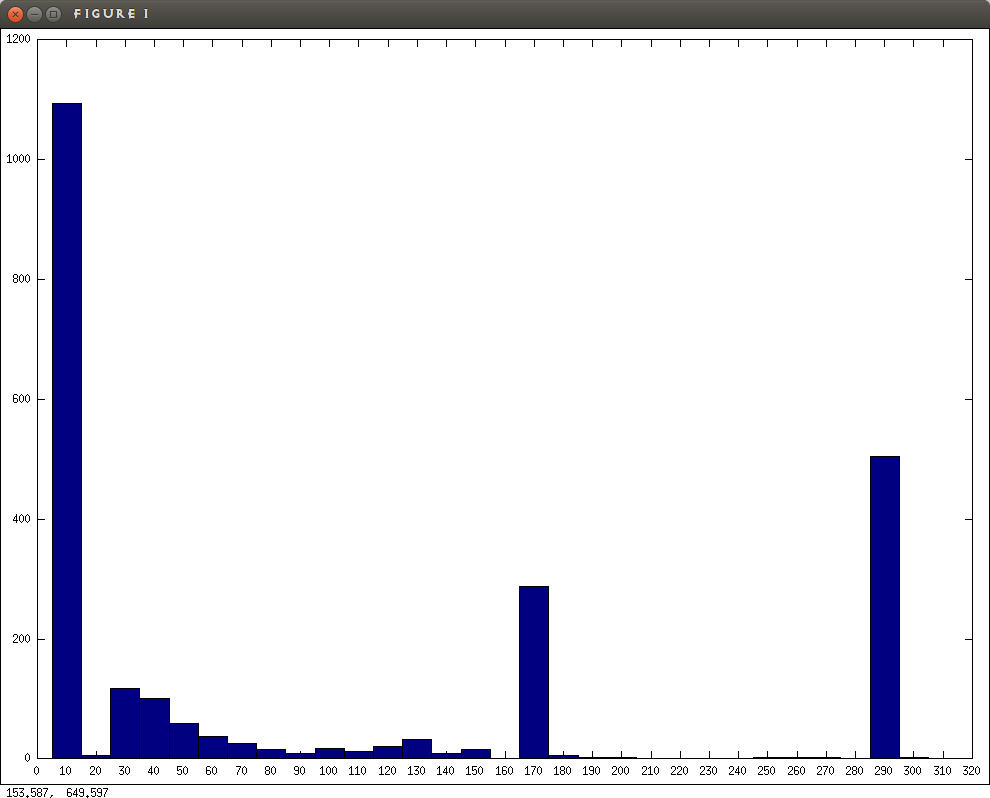
\includegraphics[width=0.5\textwidth]{fig/D_S.png}
%\caption{PING RIs of $\vec{S}_{root}$}
%\label{Fig: s_root}
%\end{figure}
%
%We then redefine $\vec{S}_{root}$ to two exclusive sub-states depends on whether the target is in a sleeping mode.
%\begin{eqnarray*}
%\vec{S}_{root} &&= \vec{S}_{sleep} + \vec{S}_{nonsleep} \\
%\vec{S}_{sleep} &&= <\text{App} = \text{RNG}, i = 5000, \text{Code} = \text{sleep}> \\
%\vec{S}_{nonsleep} &&= <\text{App} = \text{RNG}, i = 5000, \text{Code} \neq \text{sleep}>
%\end{eqnarray*}
%
%Since we know by experiment that the PING RIs are 12 to 13ms when the target is sleep; therefore we can actually approximate $\mathbb{D}_{\vec{S}_{sleep}}$ by filter out those RIs in $[12,13]$. Vice versa,  the distribution of Featured RIs can be viewed as $\mathbb{D}_{\vec{S}_{nonsleep}}$ since they are exactly the RIs filtered by the RIs of sleep. The histograms are shown in \Cref{Fig: s_sleep and s_nonsleep}.
%
%\begin{figure}
%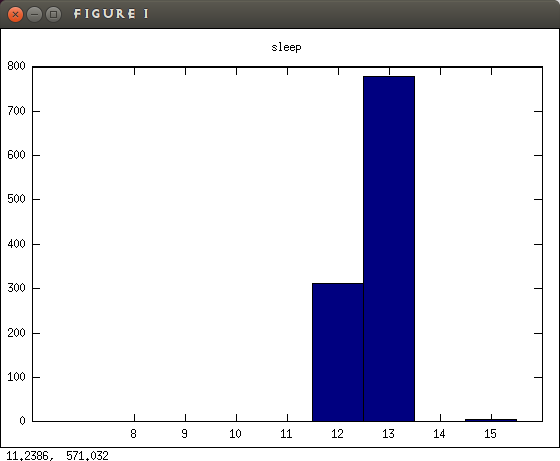
\includegraphics[width=0.5\textwidth]{fig/d_sleep.png}
%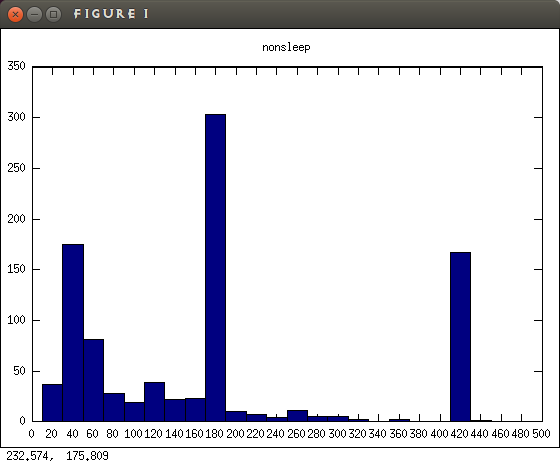
\includegraphics[width=0.5\textwidth]{fig/d_nonsleep.png}
%\caption{PING RIs of $\vec{S}_{sleep}$ and $\vec{S}_{nonsleep}$}
%\label{Fig: s_sleep and s_nonsleep}
%\end{figure}
%
%So we have
%\begin{equation} \label{Eq: sleep}
%\mathbb{D}_{\vec{S}_{main}} = p_0 \mathbb{D}_{\vec{S}_{sleep}} + p_1 \mathbb{D}_{\vec{S}_{nonsleep}}
%\end{equation}
%where $p_0$ and $p_1$ corresponds to the probability of the target being sleep and nonsleep.
%
%Solving \Cref{Eq: sleep} gives us roughly $p_0 = 0.538$ and $p_1 = 0.462$. Assuming the PING packets are received by the target randomly, we can estimate that the target is in sleep for $53.8\%$ and awake for $46.2\%$ of the time.
%
%Theoretically we can further redefine more sub-states, e.g.:
%\begin{eqnarray*}
%\vec{S}_{nonsleep} &&= \vec{S}_{RNG} + \vec{S}_{header} \\
%\vec{S}_{RNG} &&= <\text{App} = \text{RNG}, i = 5000, \text{Code} = \text{random\_rand()}> \\
%\vec{S}_{header} &&= <\text{App} = \text{RNG}, i = 5000, \text{Code} = \text{header processing}> 
%\end{eqnarray*}
%\end{example}
%
%Practically speaking, $p_i$ might be an interesting information to an  adversary as it reveals the internal state of the target which could lead to many information breach.  In practice, we might only want to approximate the solutions of $p_i$, which effectively reduces the problem of approximating \Cref{Eq: pD} to a knapsack problem\cite{knapsack}. In most cases obtaining $\mathbb{D}_{\vec{S}_i}$ is difficult as it is hard to determine the exactly the state of target sensor node at an exact moment, as in \Cref{Ex: Black Box Example}. We leave this problem to future research.

%\section{Conclusion}
In this paper we presented a study on the RNG design of CC2538. First, we revised the problem that using a 16 bit LFSR as PRNG is a bad idea and demonstrated how this design flaw can be exploited to break DTLS running on these devices. Secondly we presented a study to its seeding method and showed how such it could be remotely tampered by an adversary sending jamming signal to the device.

In fact the same RNG design has also been adopted many other products in the CC series including CC2420\cite{CC2420Manual}, CC2430\cite{CC2430Manual}, CC2520\cite{CC2520Manual} and CC253X, CC2540/41 series\cite{CC2530Manual}. We imagine all these products suffer the same problems. Fortunately the latest CC26XX/CC13XX\cite{CC26XXManual} has abandoned this design and implemented a dedicated RNG which TI describes as: (Chapter 16 in CC26XX/CC13XX Manual\cite{CC26XXManual})
\begin{quote}
The true random number generator (TRNG) module provides a true, nondeterministic noise source for the
purpose of generating keys, initialization vectors (IVs), and other random number requirements. The
TRNG is built on 24 ring oscillators that create unpredictable output to feed a complex nonlinear
combinatorial circuit. That post-processing of the output data is required to obtain cryptographically secure
random data.
\end{quote}

We sincerely hope this TRNG will provide the future IoT applications a secure RNG.

\section{Acknowledgement}
We have many thanks to (alphabetically) George Oikonomou for providing us much help in Contiki OS and the OpenMote devices, Geoff Hilton who helped us on RF designs and Jake Longo Galea who offered many signal processing advises.
\appendix
\chapter{OrderFlavour-Length leakage channel}
\label{OrderFlavour leakage channel}

In this application, the joint probability of $Order$ and $Flavour$ are simply the product of their marginal probability. However, since “ESPRESSO” will always followed by $Flavour$ of of both degree of SUGAR and MILK being $0$(see  \Cref{ESPRESSO}); hence
\begin{eqnarray*}
P(x_1, x_2 | \text{“ESPRESSO”}) = 
	\begin{cases}
	1 &\text{if } x_1 = x_2 = 0\\
	0 &\text{otherwise}
	\end{cases}
\end{eqnarray*}

Therefore
\begin{eqnarray*}
P(\text{“ESPRESSO”}, x_1, x_2 ) = 
	\begin{cases}
	1/4 &\text{if } x_1 = x_2 = 0\\
	0 &\text{otherwise}
	\end{cases}
\end{eqnarray*}

%Bibliographies
\bibliography{references,rfc}
\bibliographystyle{ieeetr}

%\printbibliography

\end{document}
